\documentclass{article}
\usepackage{amsmath}
\usepackage{graphicx} 
\usepackage{float}
\usepackage{caption}


\begin{document}


\section{Eficiência de grids/torus $n \times m$}
Começamos sem analisar redes complexas, criando um código em C++ puro (sem bibliotecas) com roteamento implementado do zero, para facilitar a análise fizemos um grid $n \times m$, vendo como a proporção $n/m$ e a taxa da geração de mensagens $p$ influenciava na eficiência da rede.

\subsection{Razão $n/m$}
Como o esperado, grids com razões mais próximos de 1, ou seja, próximo de quadrados, tinham maior eficiência

\begin{figure}[H]
    \centering
    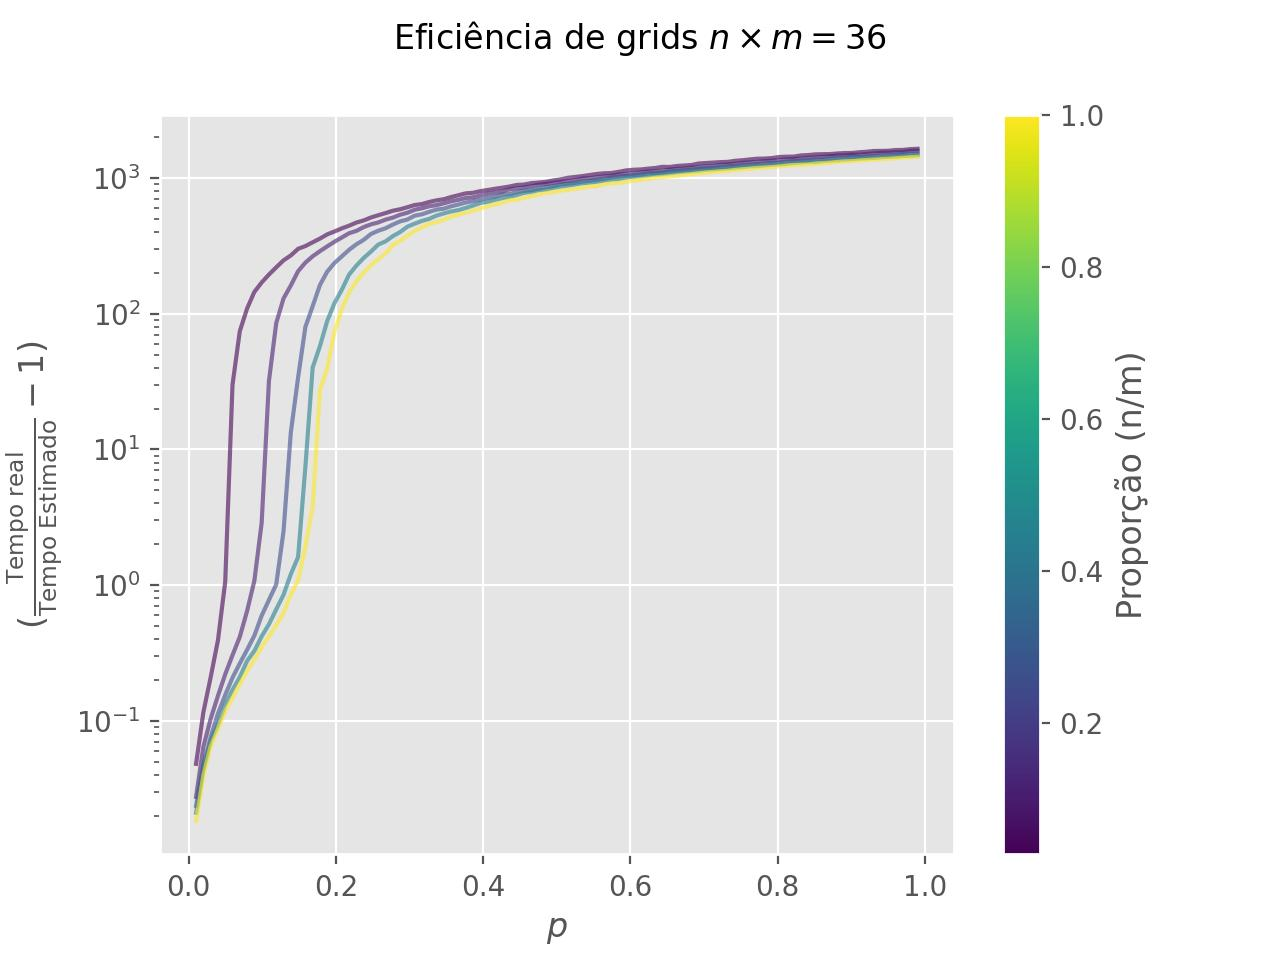
\includegraphics[width=0.8\linewidth]{images/razoes_N36_grid.jpg}
    \caption{Diferentes razões n/m no grid }
    \label{fig:enter-label}
\end{figure}


\subsection{Grid vs Torus}
Quando comparamos a topologia de um torus com um grid observamos que o torus é bem mais eficiente, o que faz sentido visto a menor distância média entre dois pontos

\begin{figure}[H]
    \centering
    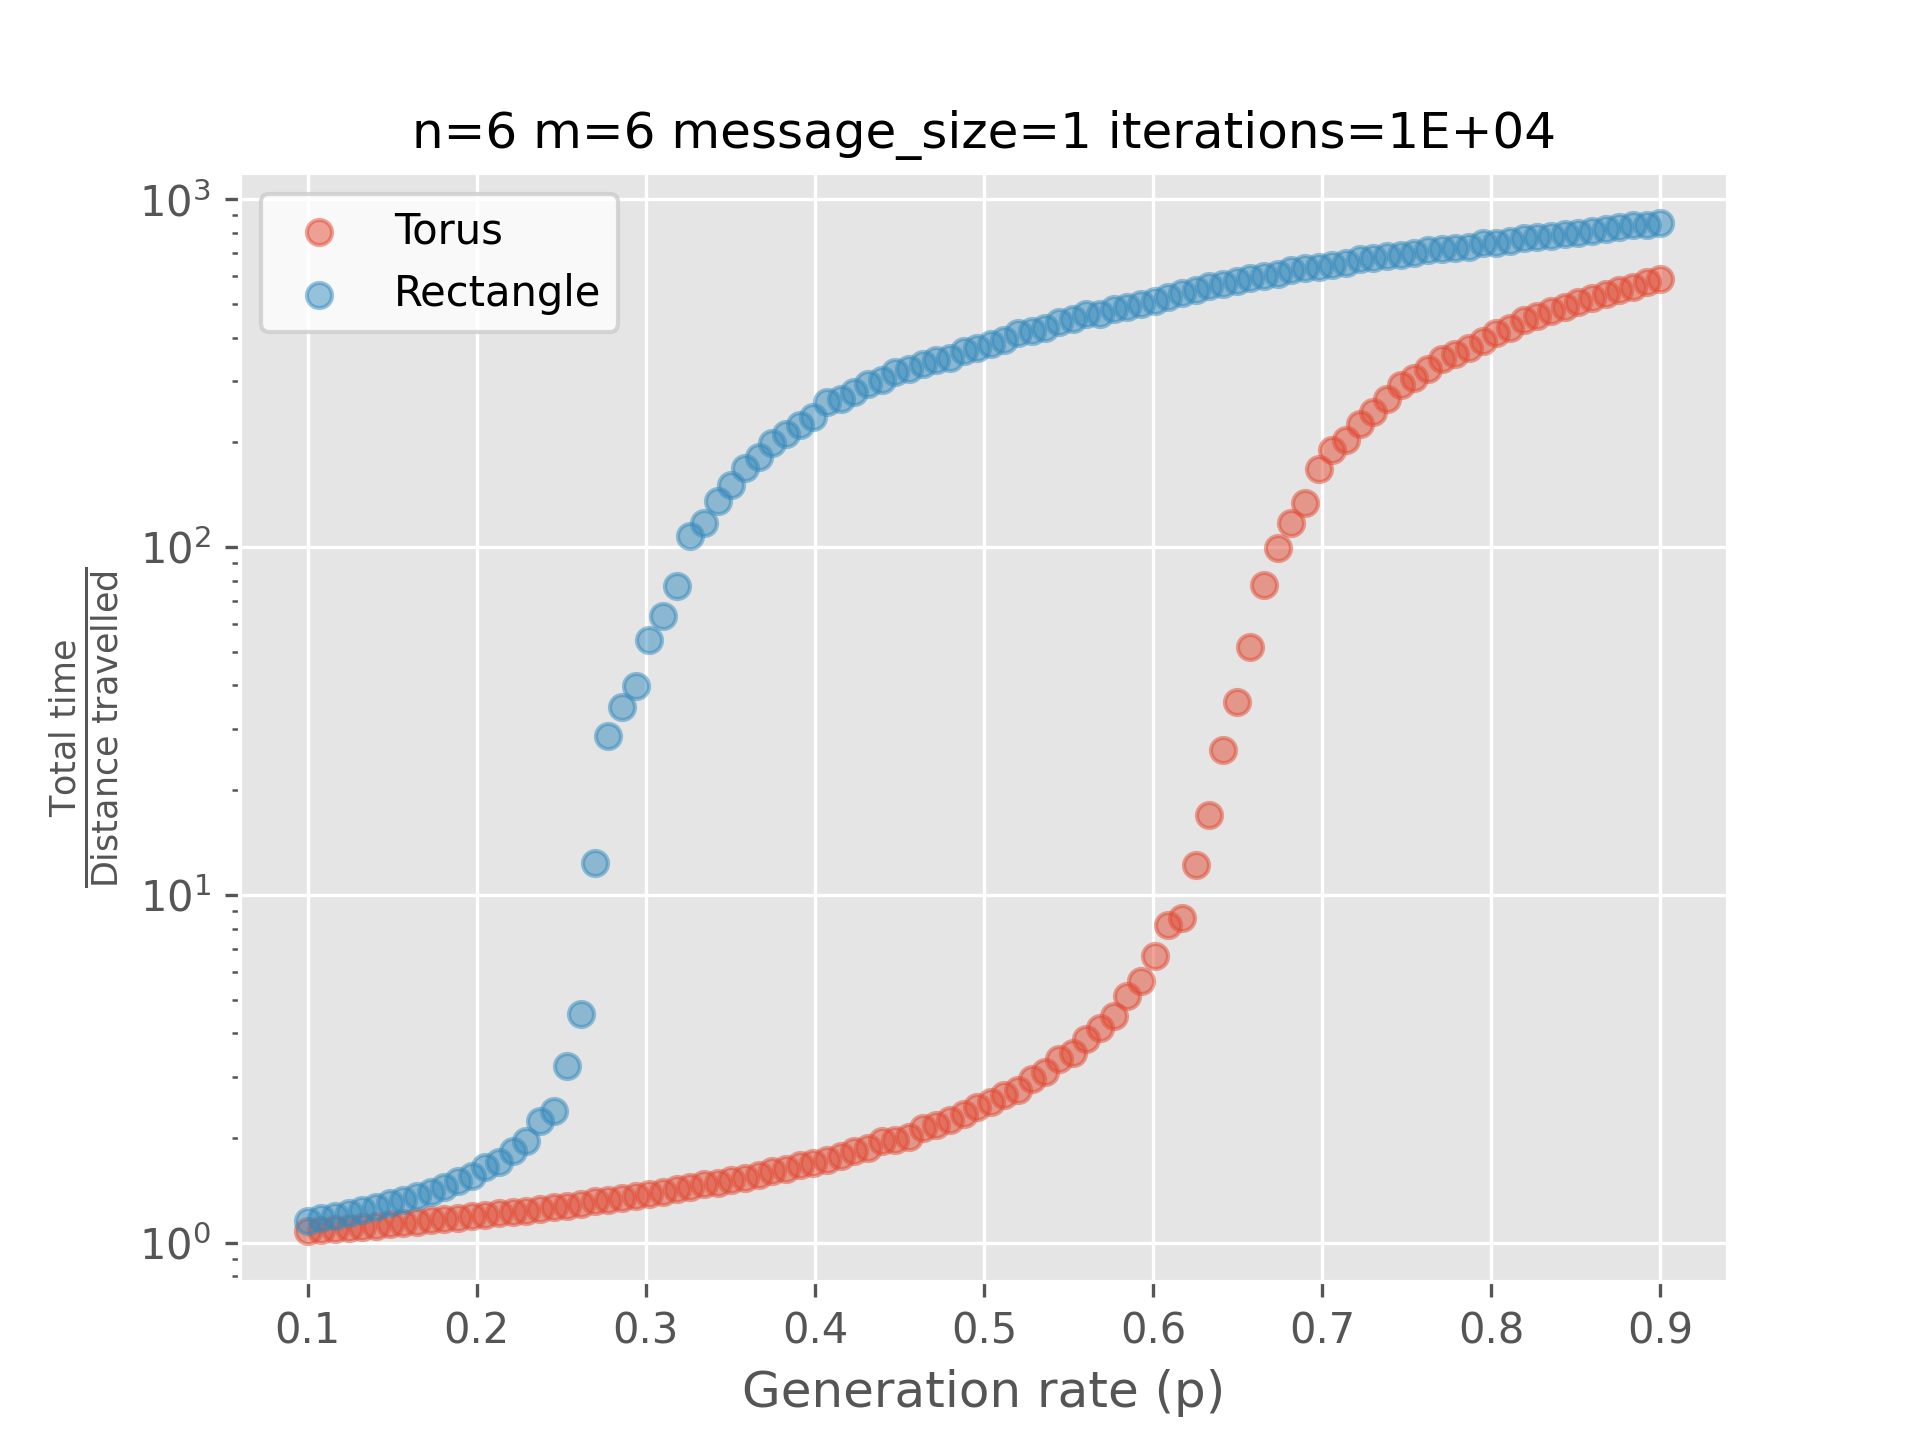
\includegraphics[width=0.8\linewidth]{images/torus_vs_grid.png}
    \caption{torus vs grid }
    \label{fig:enter-label}
\end{figure}

%% p vs eficiencia
%% média temporal de mensagens vs betweenneess centrality

\section{Fitting do $p_{critico}$}
Fizemos várias tentativas para encontrar uma estimativa para a transição de fase do estado estável para o crítico, mesmo que uma transição de fase seja difícil caracterizar é interessante observar o que conseguimos fazer.

\subsection{Relação com o coeficiente de Pearson}
No estado crítico o número de mensagens cresce linearmente com o tempo, então é a razoável que o coeficiente de Pearson (Número de mensagens x Tempo) seja próximo de 1 no estado crítico. Devido a termos usados diferentes instâncias do mesmo modelo, o p não correlacionou bem nas figuras

\begin{figure}[H]
    \centering
    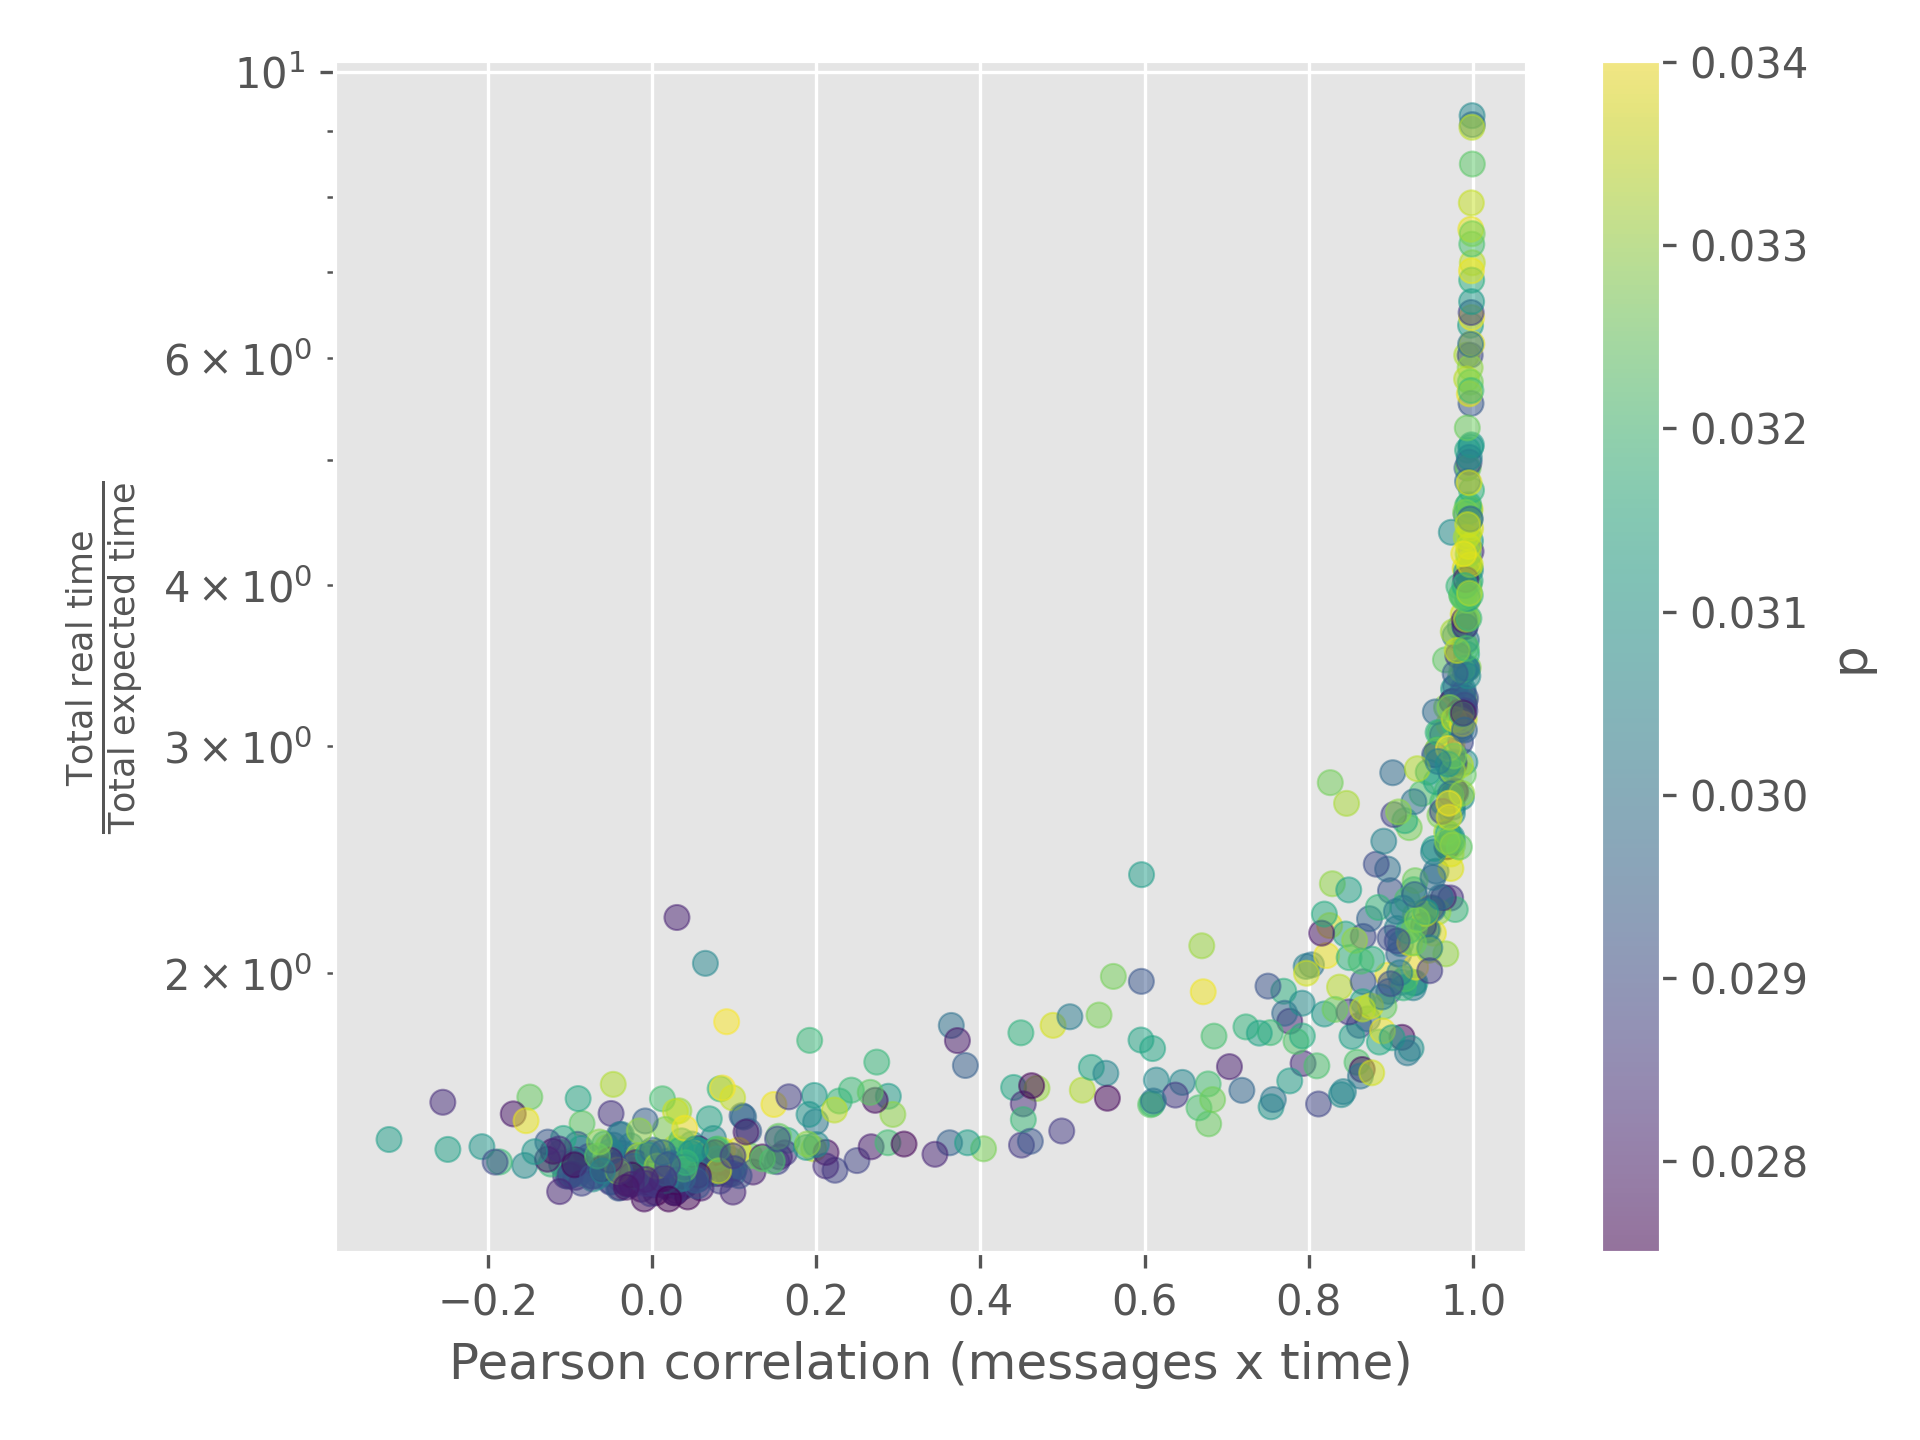
\includegraphics[width=0.8\linewidth]{images/p_critico_barabasi.png}
    \caption{Barabási e número de mensagens}
    \label{fig:enter-label}
\end{figure}


\begin{figure}[H]
    \centering
    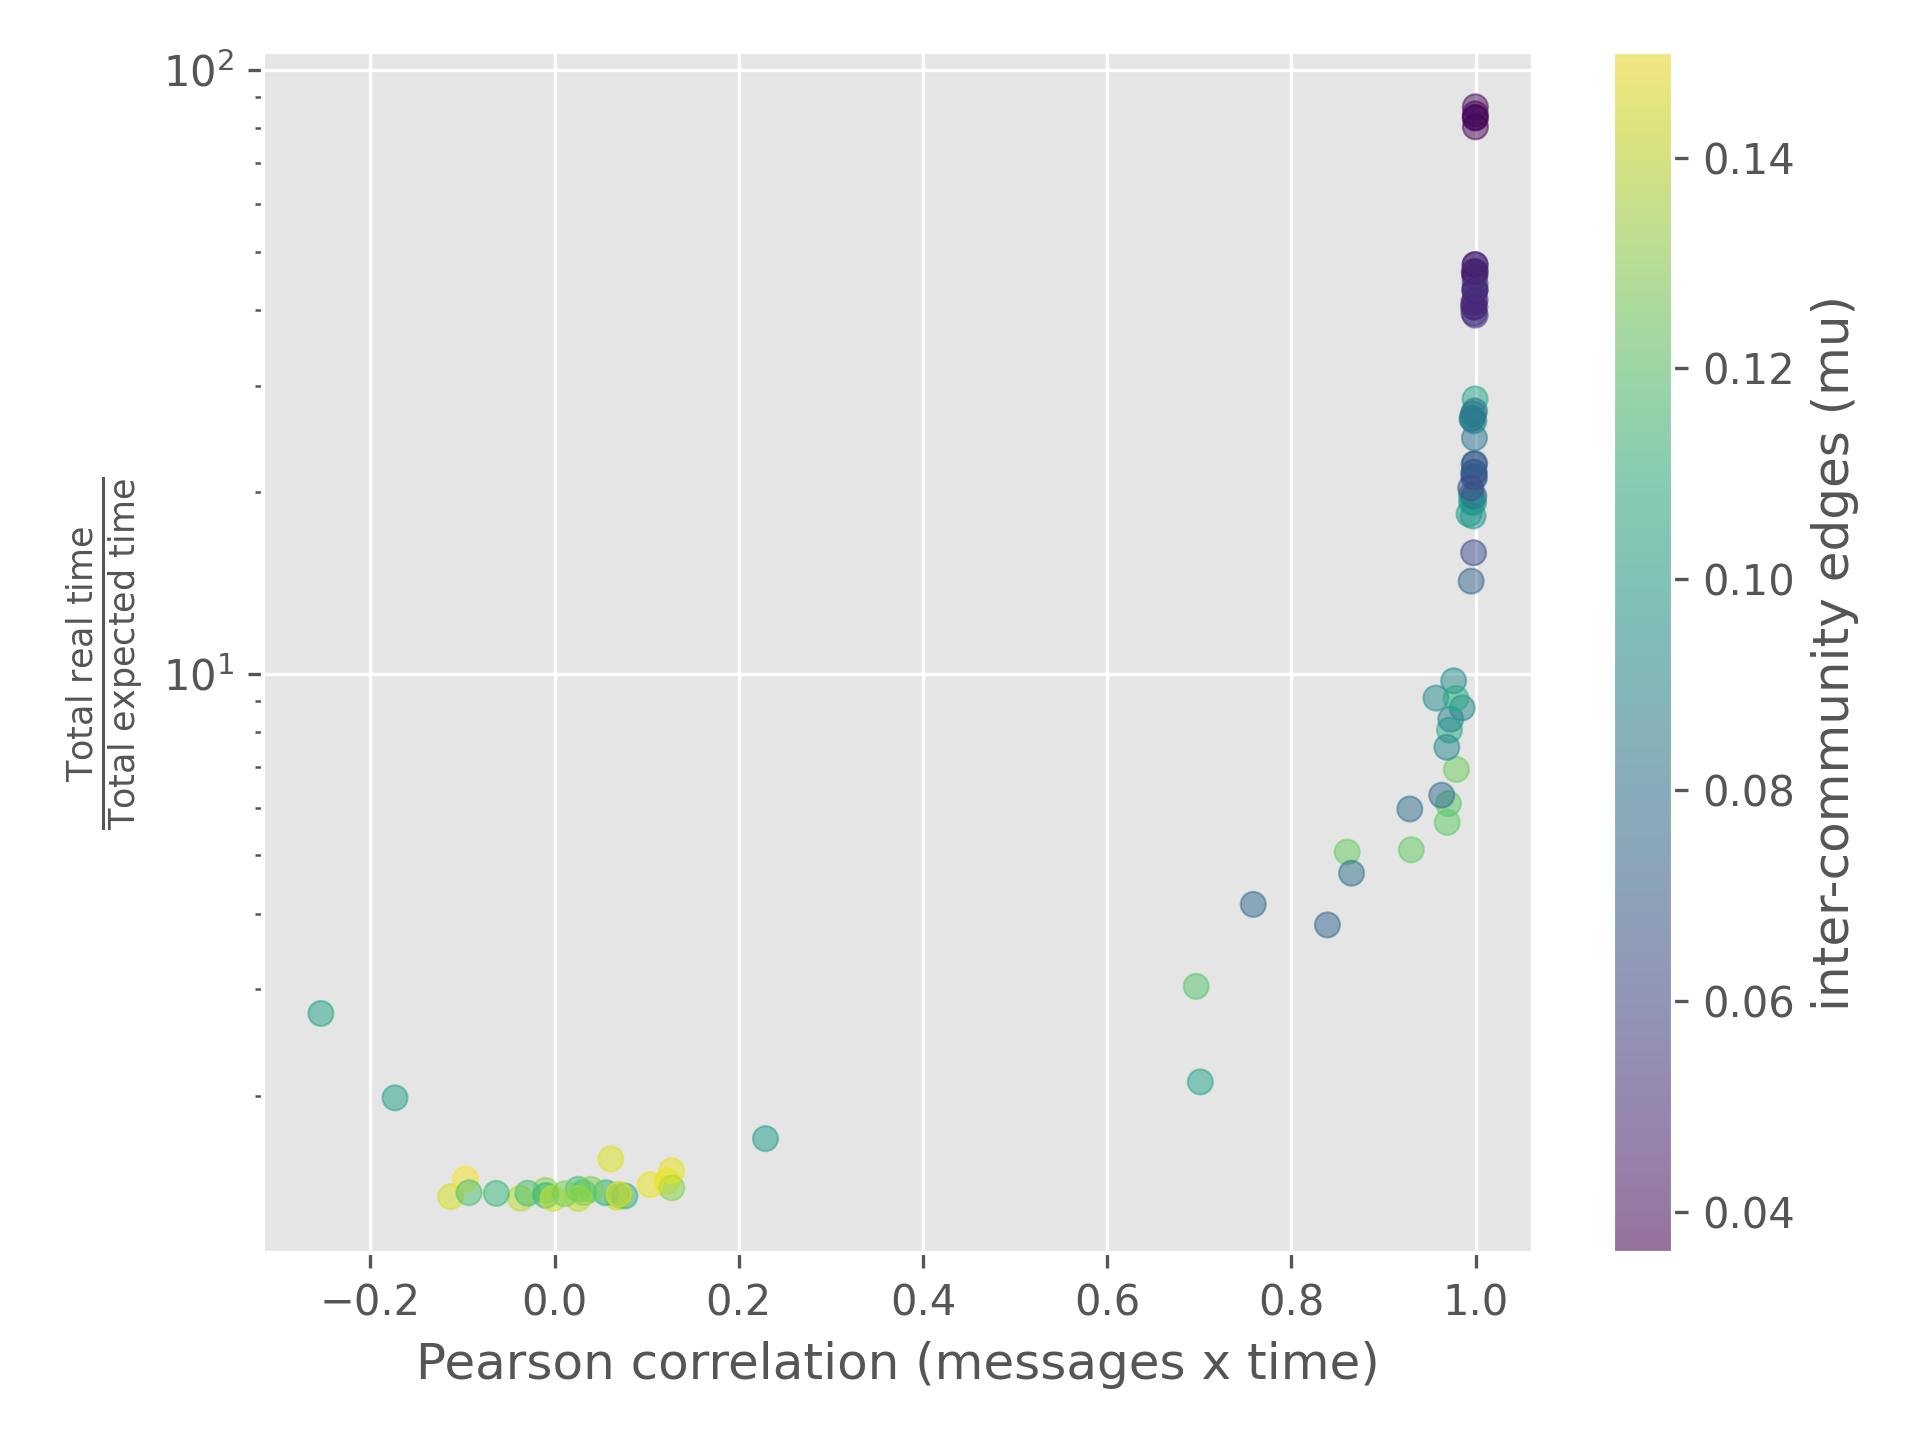
\includegraphics[width=0.8\linewidth]{images/p_critico_lfr.png}
    \caption{LFR e número de mensagens}
    \label{fig:enter-label}
\end{figure}

\subsection{Forma fechada}
Para um caso mais simples conseguimos achar uma boa estimava para $p_{critico}$, ela foi usada especificamente no caso de grids e torus, a ideia é que no estado crítico o número de mensagens gerados é igual ao número de mensagens entregues

\begin{equation}
(n \times m) \times p_{critico}= \frac{(n \times m)}{L_G}     
\end{equation}

Chegando na conclusão que $p_{critico}=\frac{1}{L_G}$

\begin{figure}[H]
    \centering
    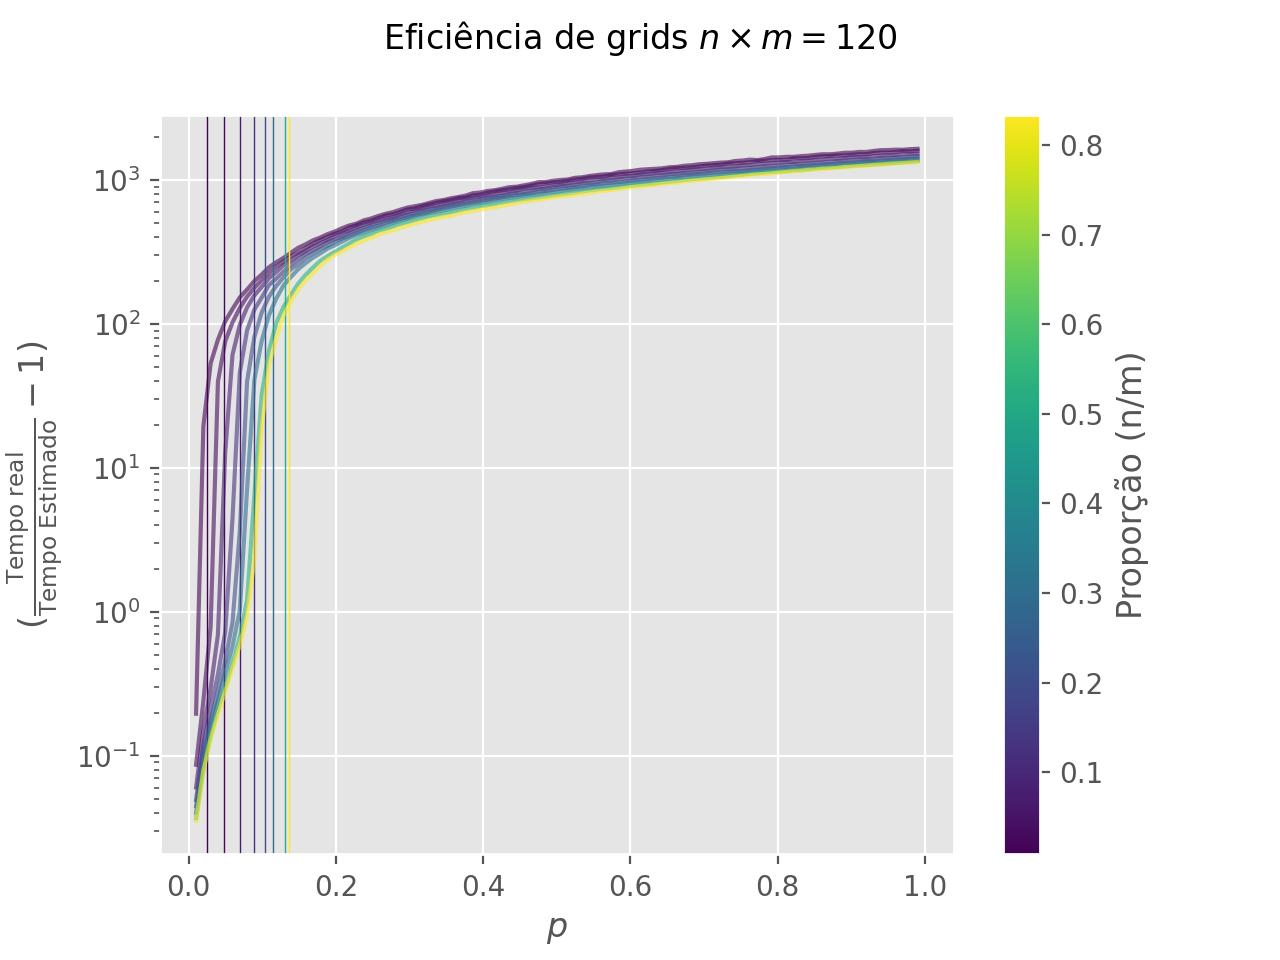
\includegraphics[width=0.8\linewidth]{images/p_critico_grid_120.jpg}
    \caption{Estimando $p_{critico}$ grid $N=120$ }
    \label{fig:enter-label}
\end{figure}


\begin{figure}[H]
    \centering
    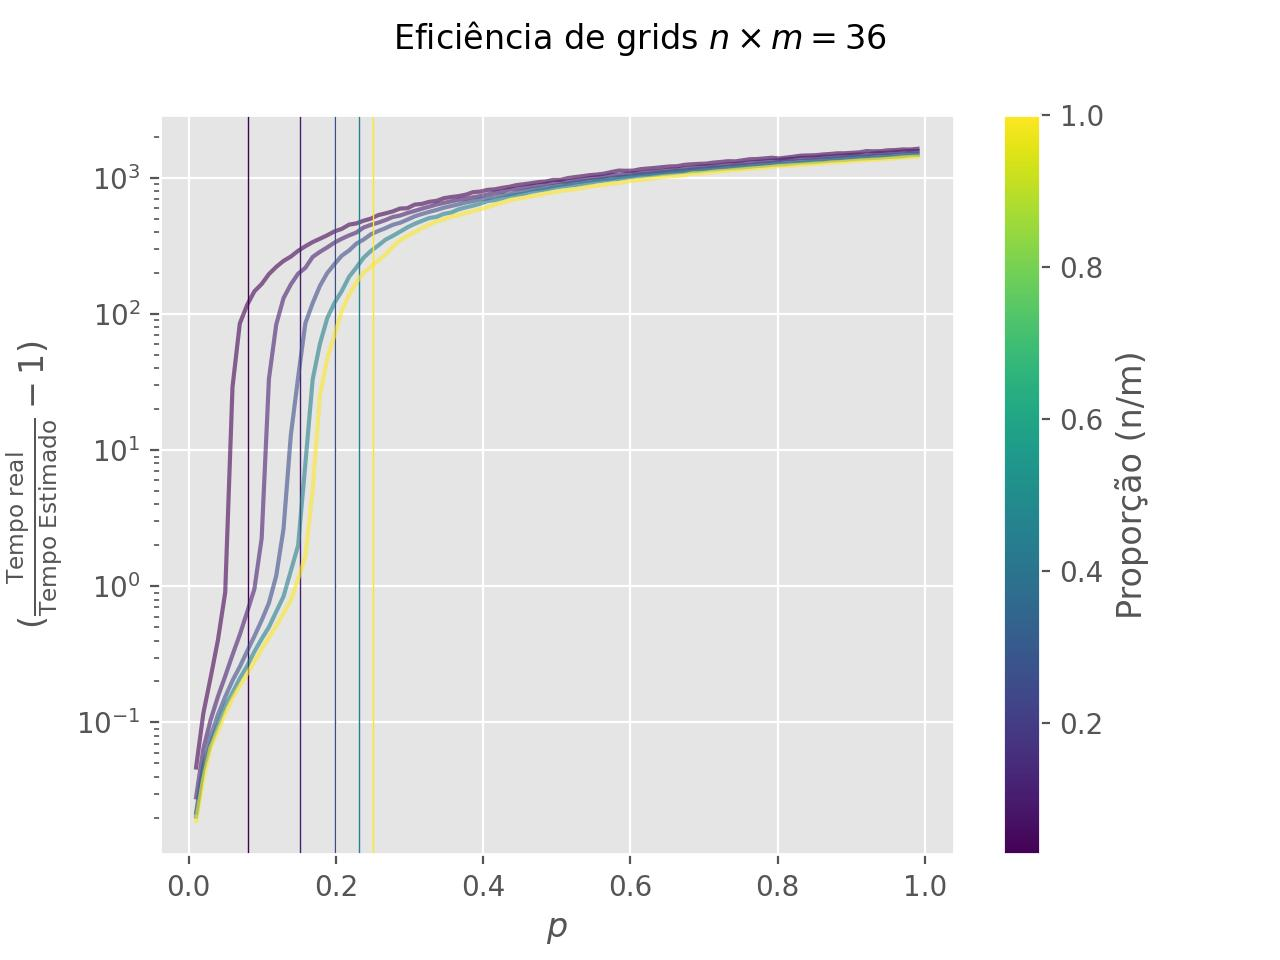
\includegraphics[width=0.8\linewidth]{images/p_critico_grid36.jpg}
    \caption{Estimando $p_{critico}$ grid $N=36$ }
    \label{fig:enter-label}
\end{figure}






\section{Roteamento com visibilidade limitada}
Analisamos como o roteamento em uma rede Barabási era impactado considerando que a partir de uma distância máxima $D$, o roteamento seria feito aleatoriamente para um vértice vizinho.

\begin{figure}[H]
    \centering
    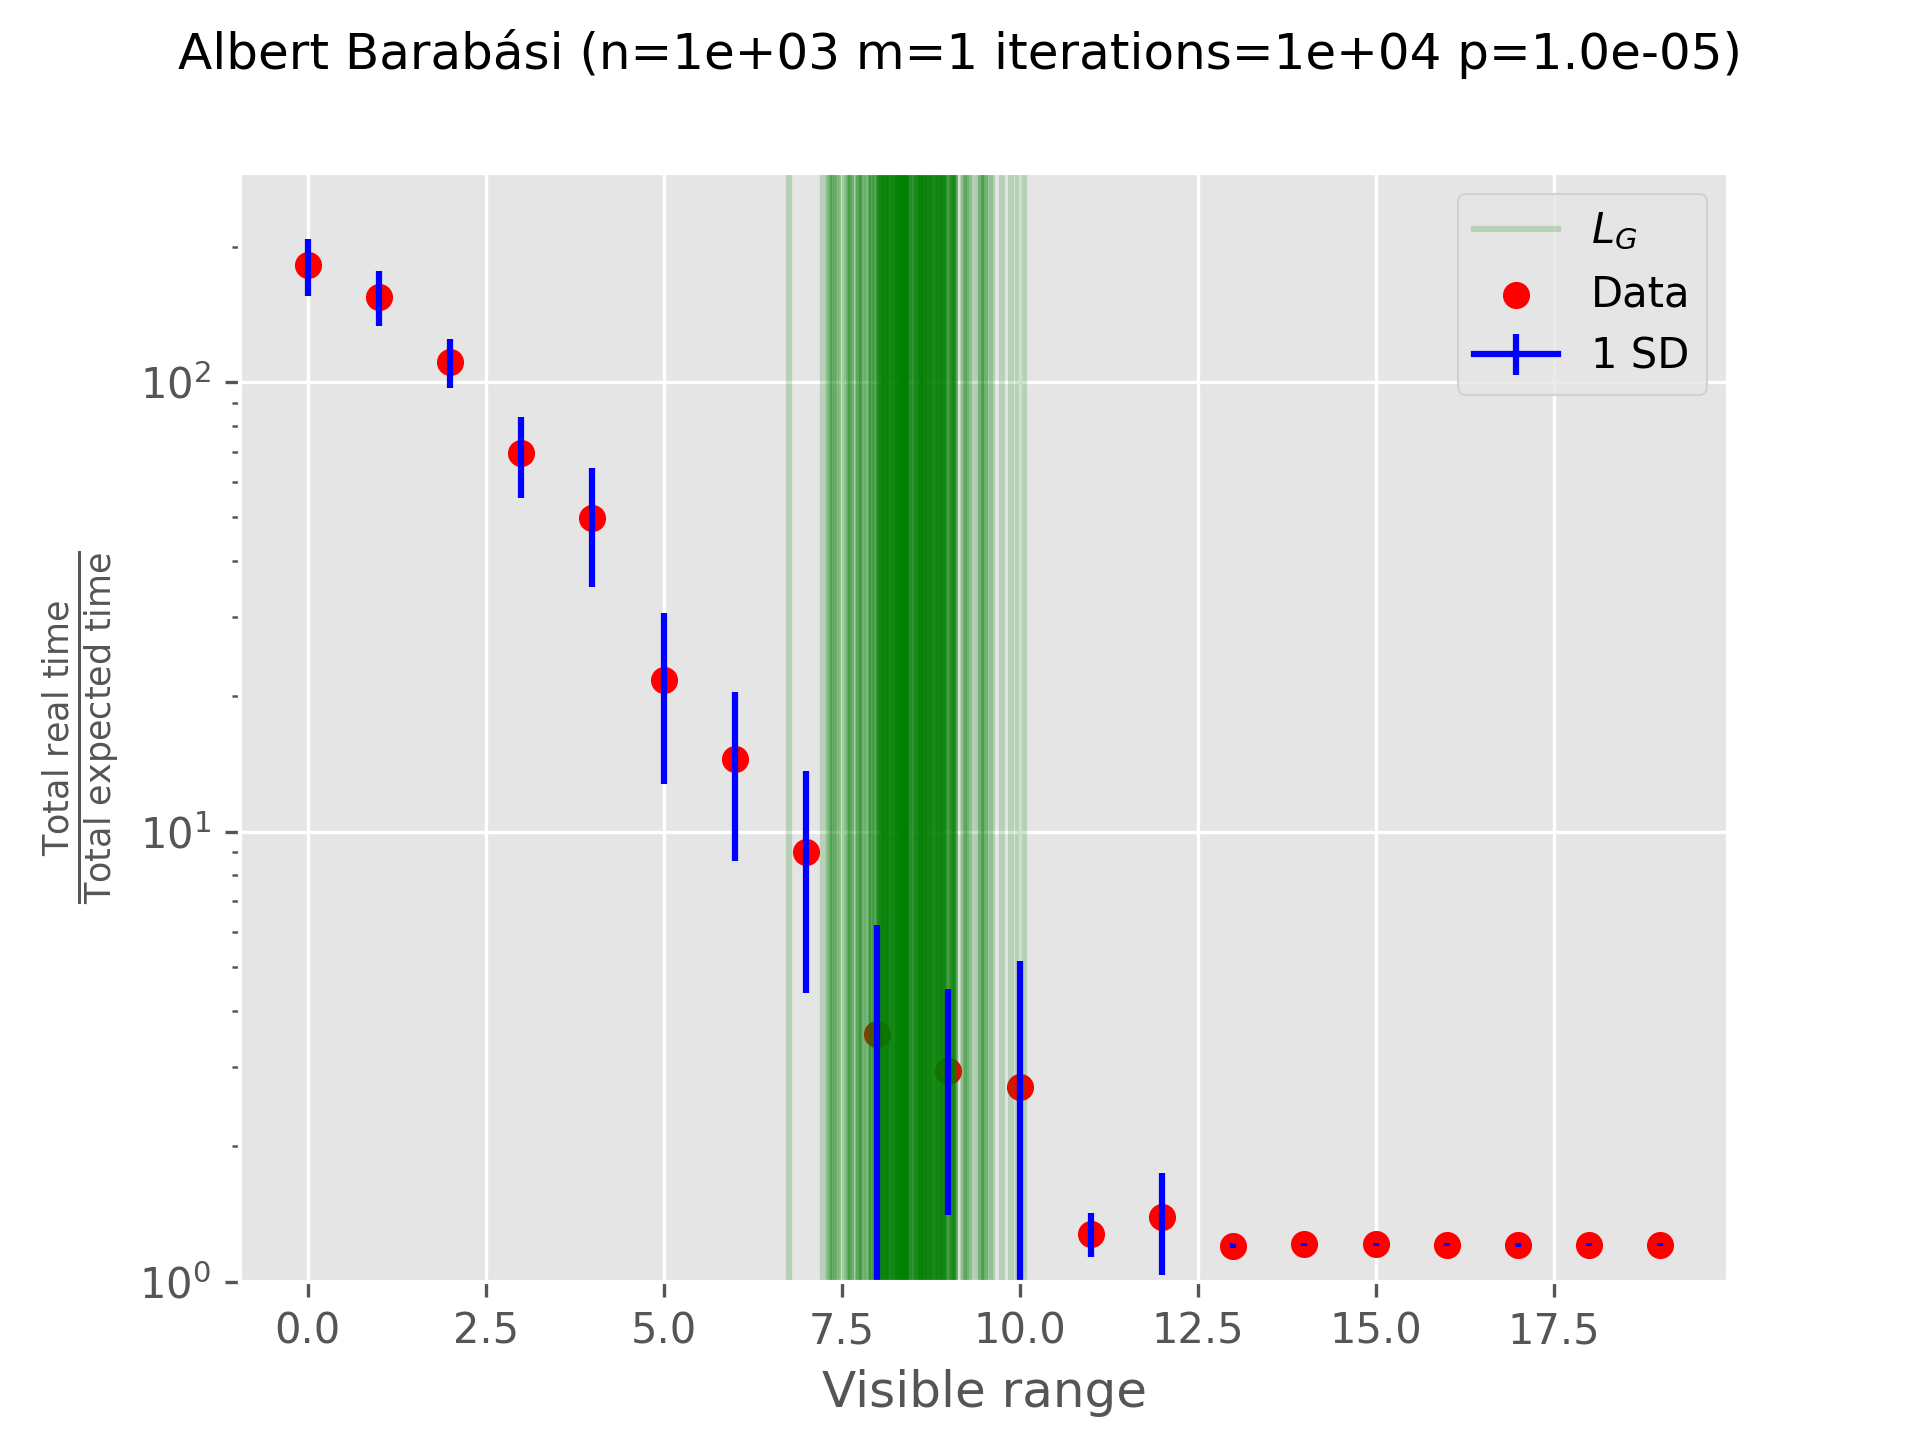
\includegraphics[width=0.8\linewidth]{images/visible_m1.png}
    \caption{Barabási $m=1$ visibilidade limitada }
    \label{fig:enter-label}
\end{figure}

Obviamente a eficiência do sistema cresce quando a visibilidade aumenta, porque o roteamento é feito por caminhos mínimos e não por um caminho aleatório. As linhas verticais indicam a média de todos os caminhos mínimos do grafo, já como fizemos repetições para termos uma significância estatística, são várias linhas.

A ideia é que cada mensagem só precisa em média ter um roteamento com visibilidade $L_G$, então é esperado que para $D>L_G$ a eficiência esteja próximo do ótimo


\begin{figure}[H]
    \centering
    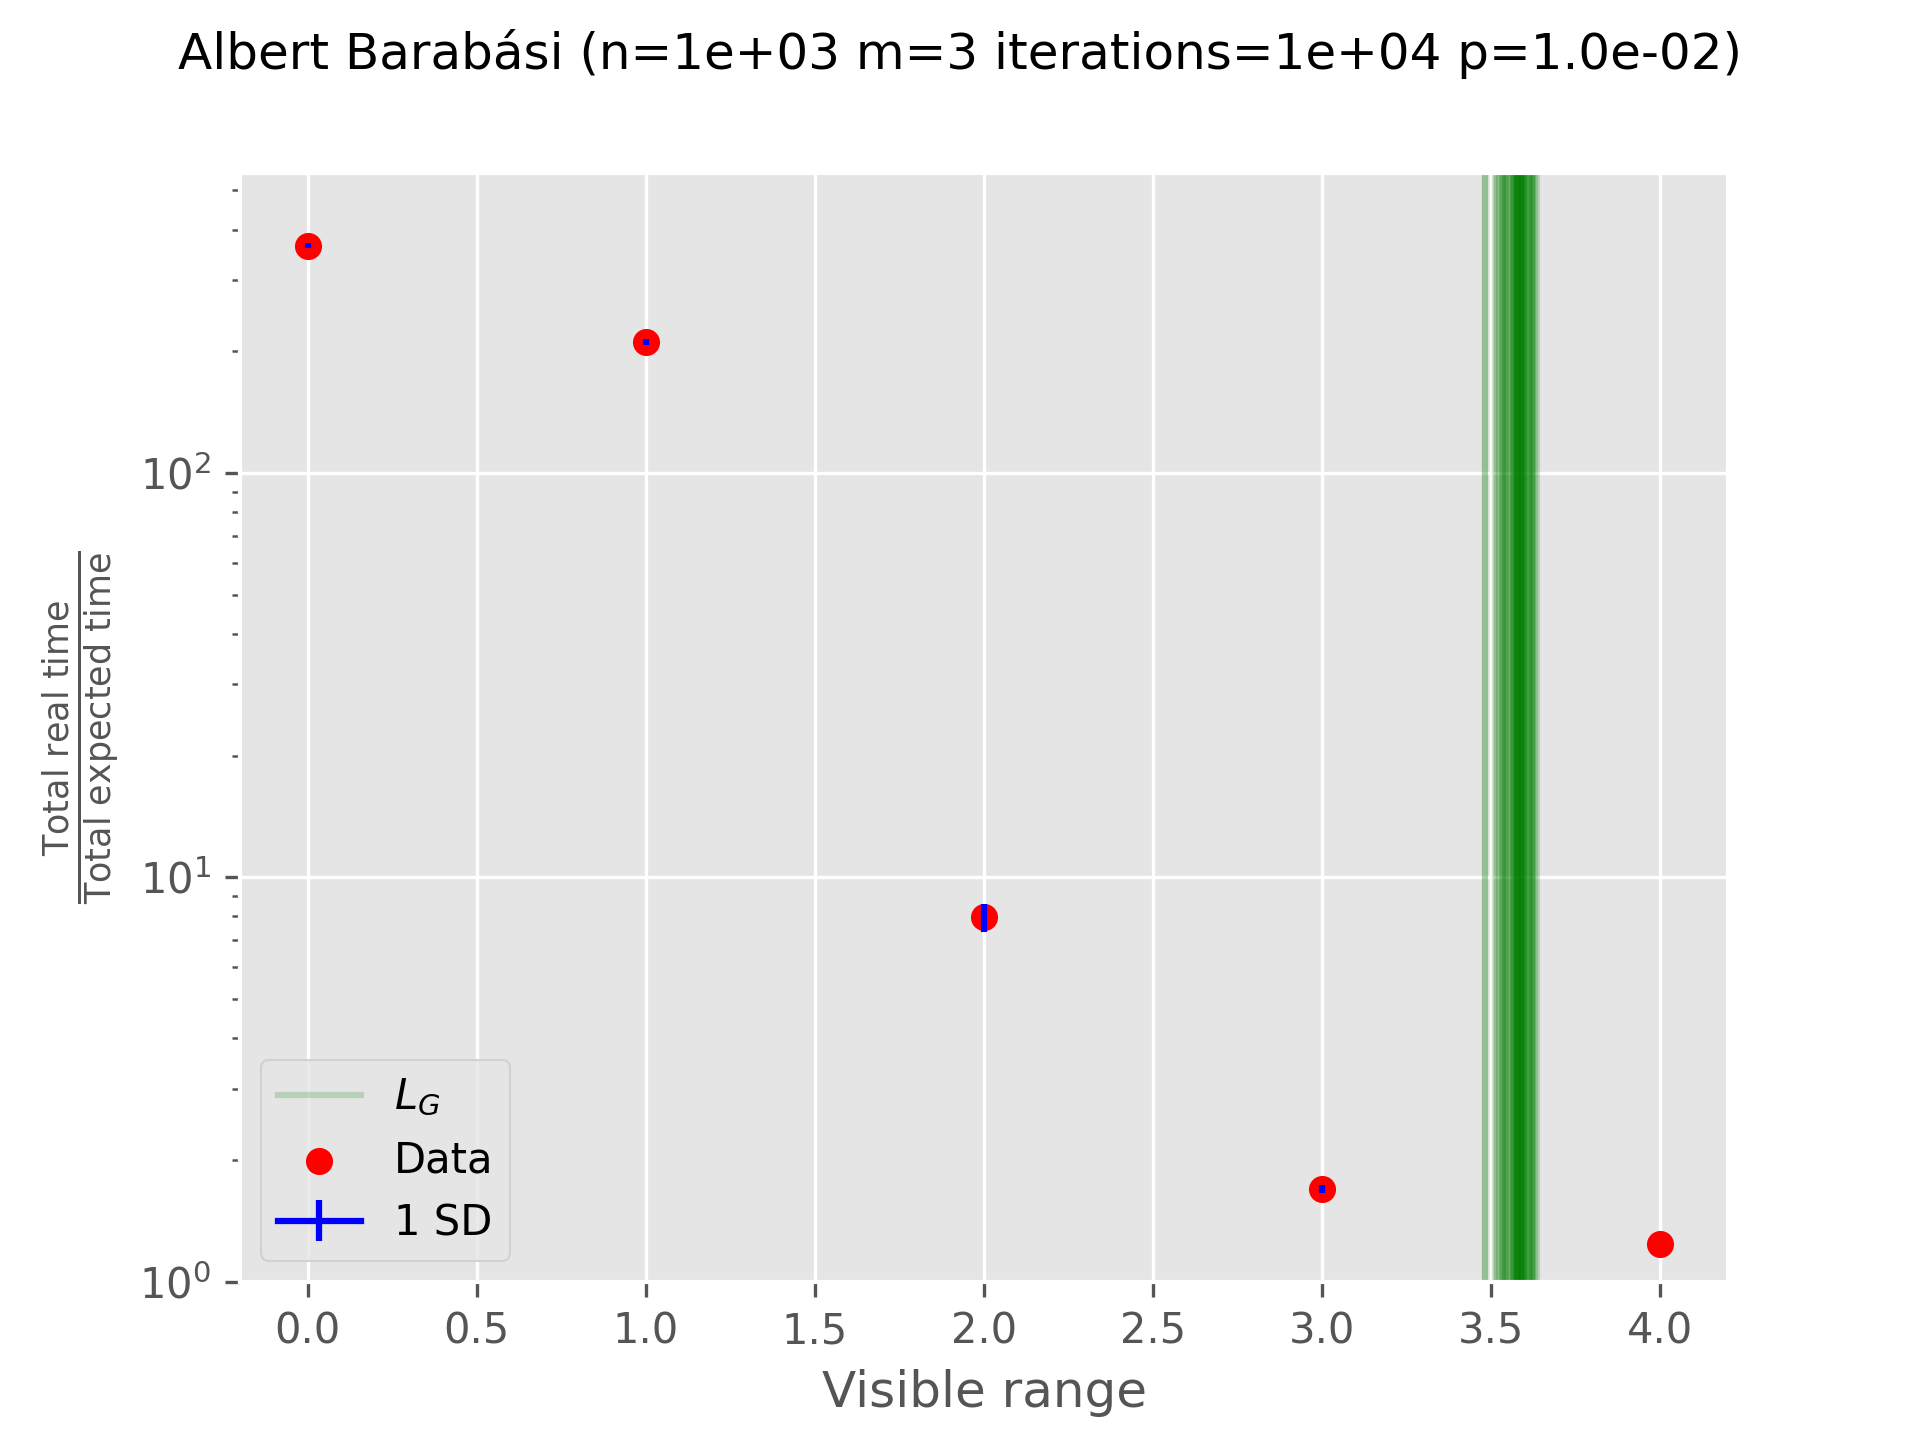
\includegraphics[width=0.8\linewidth]{images/visible_m3.png}
    \caption{Barabási $m=3$ visibilidade limitada }
    \label{fig:enter-label}
\end{figure}

\begin{figure}[H]
    \centering
    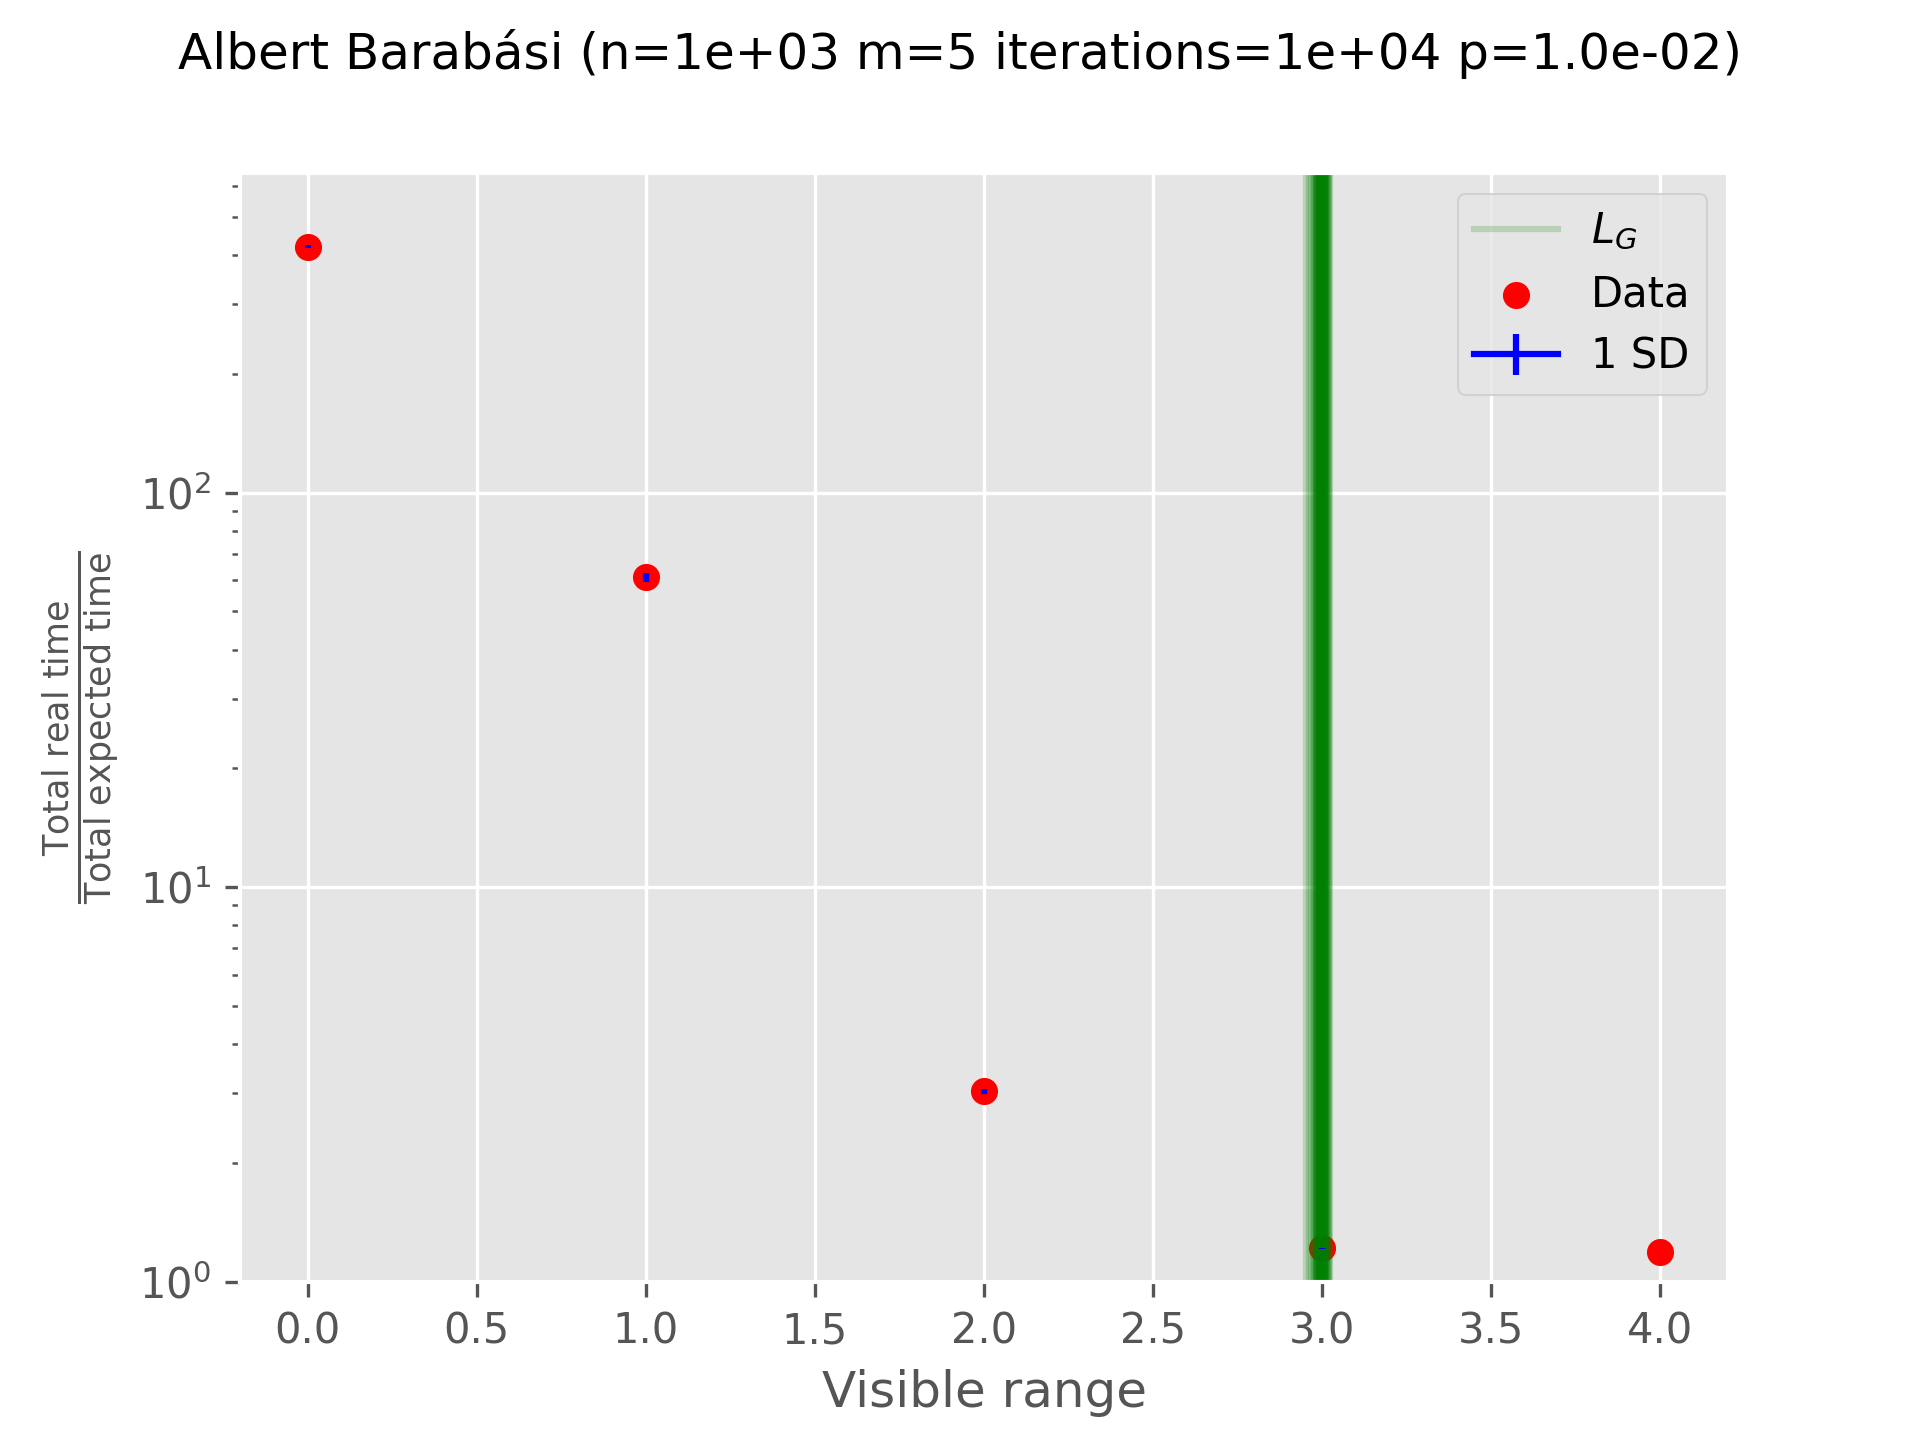
\includegraphics[width=0.8\linewidth]{images/visible_m5.png}
    \caption{Barabási $m=5$ visibilidade limitada }
    \label{fig:enter-label}
\end{figure}







\section{LFR Benchmark}
Observamos que no modelo LFR a eficiência está muito relacionada com o grau de conexão entre comunidades, se uma mensagem precisa ir de uma comunidade para outra,um baixo inter-community fraction diminui muito a eficiência da rede. Acima de um valor crítico não se observa melhoras significativas
\begin{figure}[H]
    \centering
    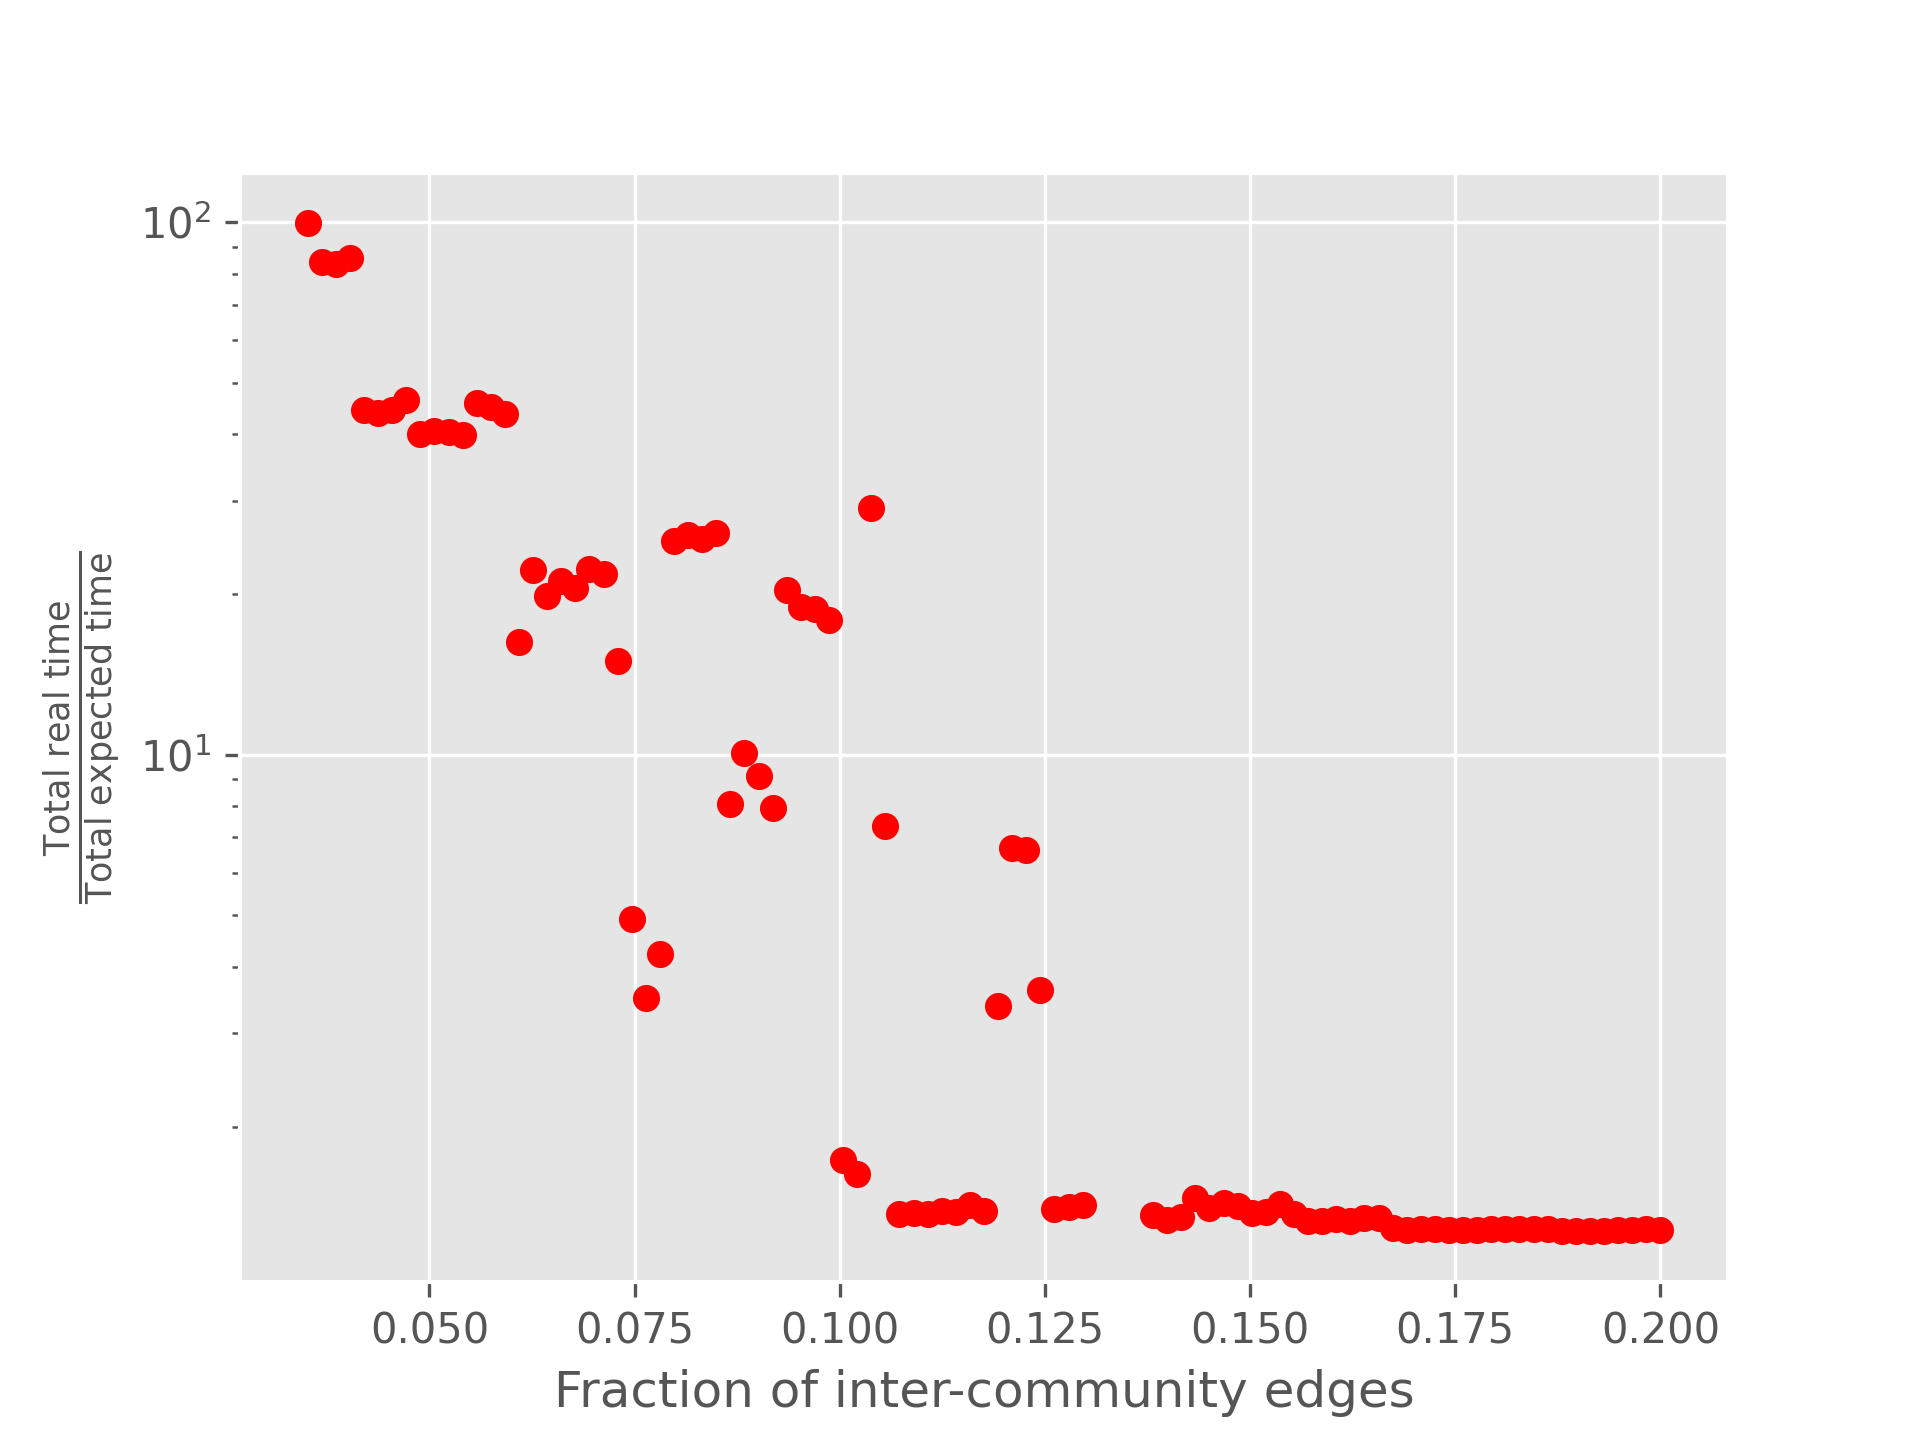
\includegraphics[width=0.8\linewidth]{images/lfr.png}
    \caption{LFR com diferentes graus de conexão entre comunidades }
    \label{fig:enter-label}
\end{figure}

\section{(MÉTODO ANTIGO) Otimização do número de conexões}
Vamos tentar encontrar um número mínimo de conexões em uma certa topologia tal que o tráfego em cada conexão não seja maior que um dado valor $k$, começamos inicialmente com todas as conexões com largura de banda unitária, caso o número de mensagens ultrapasse $k$, aumentamos a largura de banda em uma unidade.

\begin{equation}
    \text{Largura de banda}=\frac{\text{Quantidade de dados}}{\text{Iterações}}
\end{equation}

\subsection{(MÉTODO ANTIGO) Barabási}

Quando analisamos a distribuição de largura de banda, vemos que ela se correlaciona com a edge betweenness de cada conexão, para certos intervalos se observa uma lei de potência. O que faz sentido, conexões mais centrais exigem uma largura de banda maior para não se congestionarem.



Analisamos o estado transiente e estacionário do algoritmo, o número de mensagens atinge um pico e depois oscila aleatoriamente em torno de uma média, tentamos fazer um fitting considerando um caso sem nenhum congestionamento


\begin{figure}[H]
    \centering
    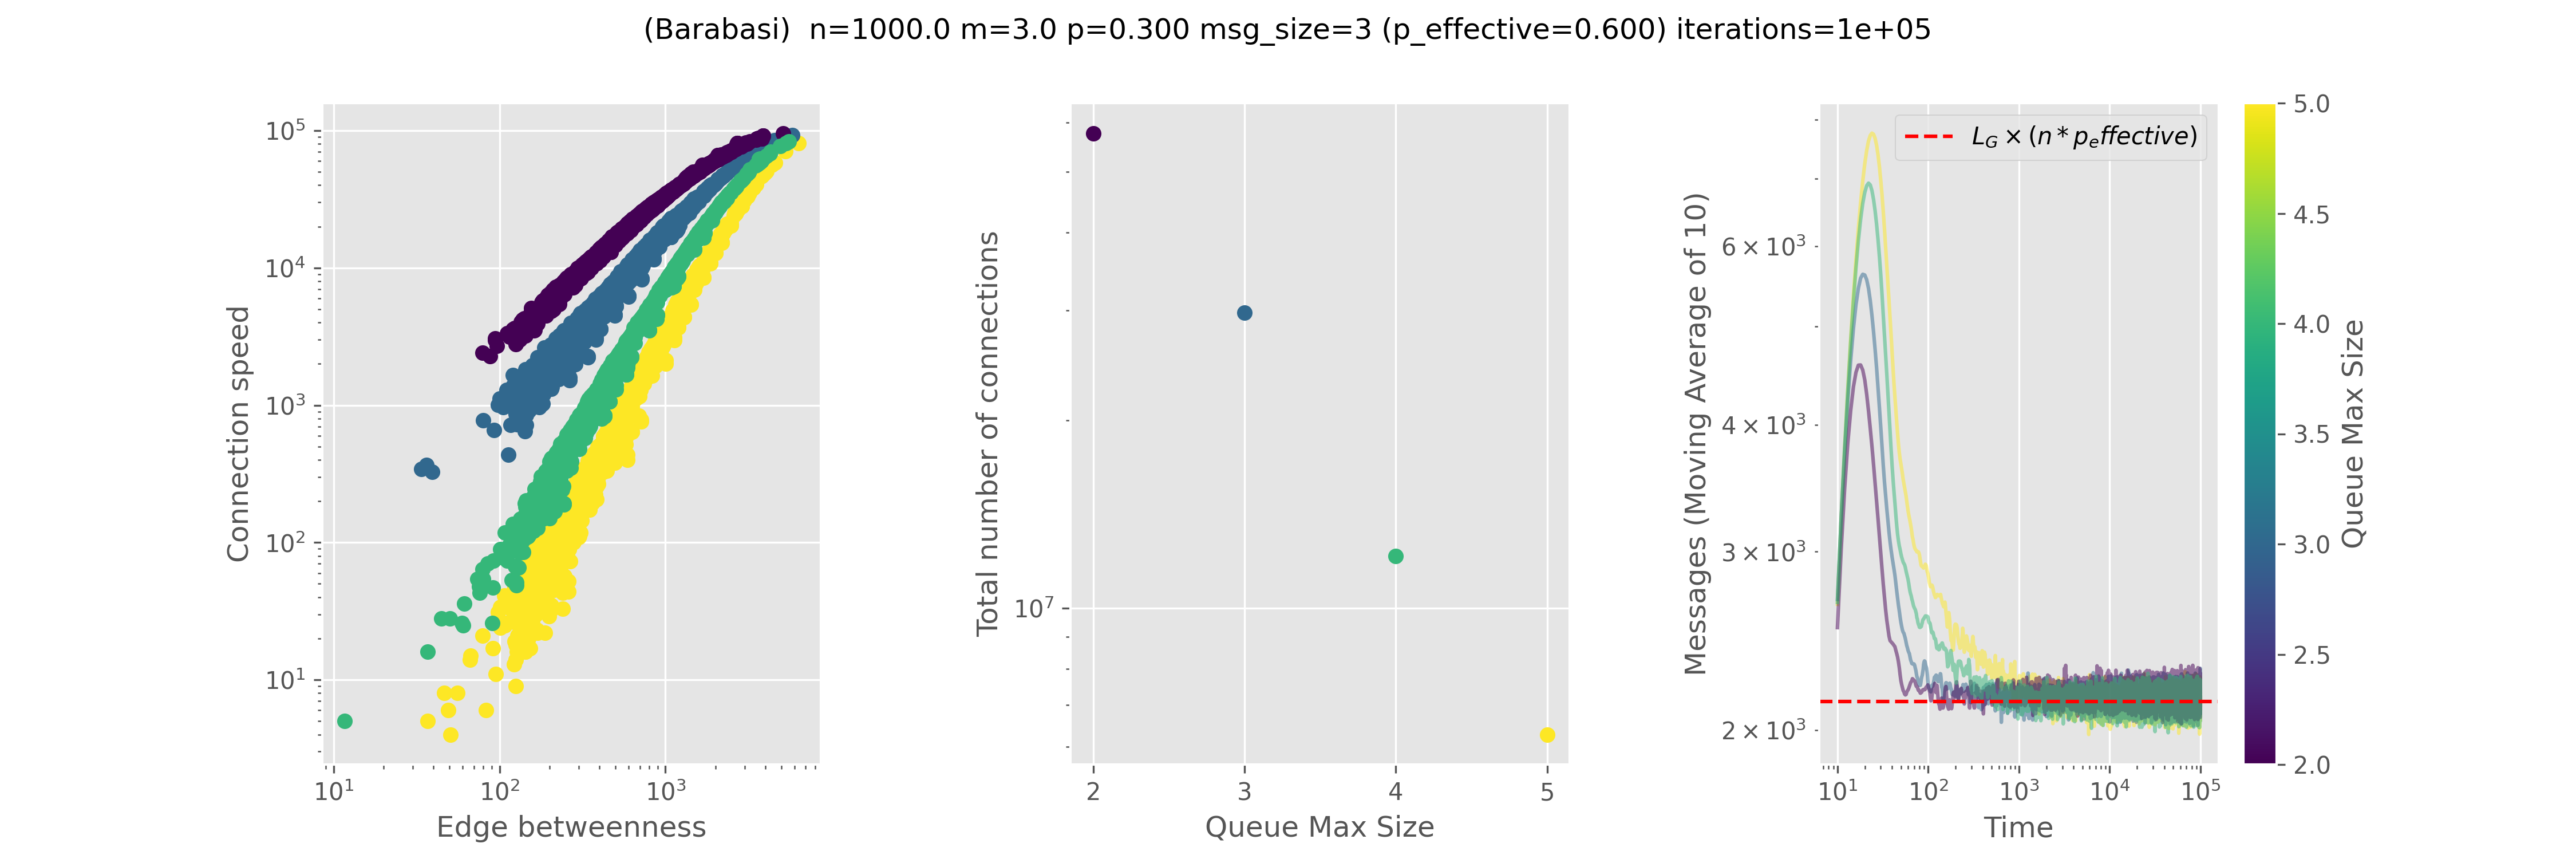
\includegraphics[width=0.8\linewidth]{images/queue_max_size/barabasi_queue_2-5.png}
    \caption{Barabási otimização $k=[2,5]$ }
    \label{fig:enter-label}
\end{figure}


\begin{figure}[H]
    \centering
    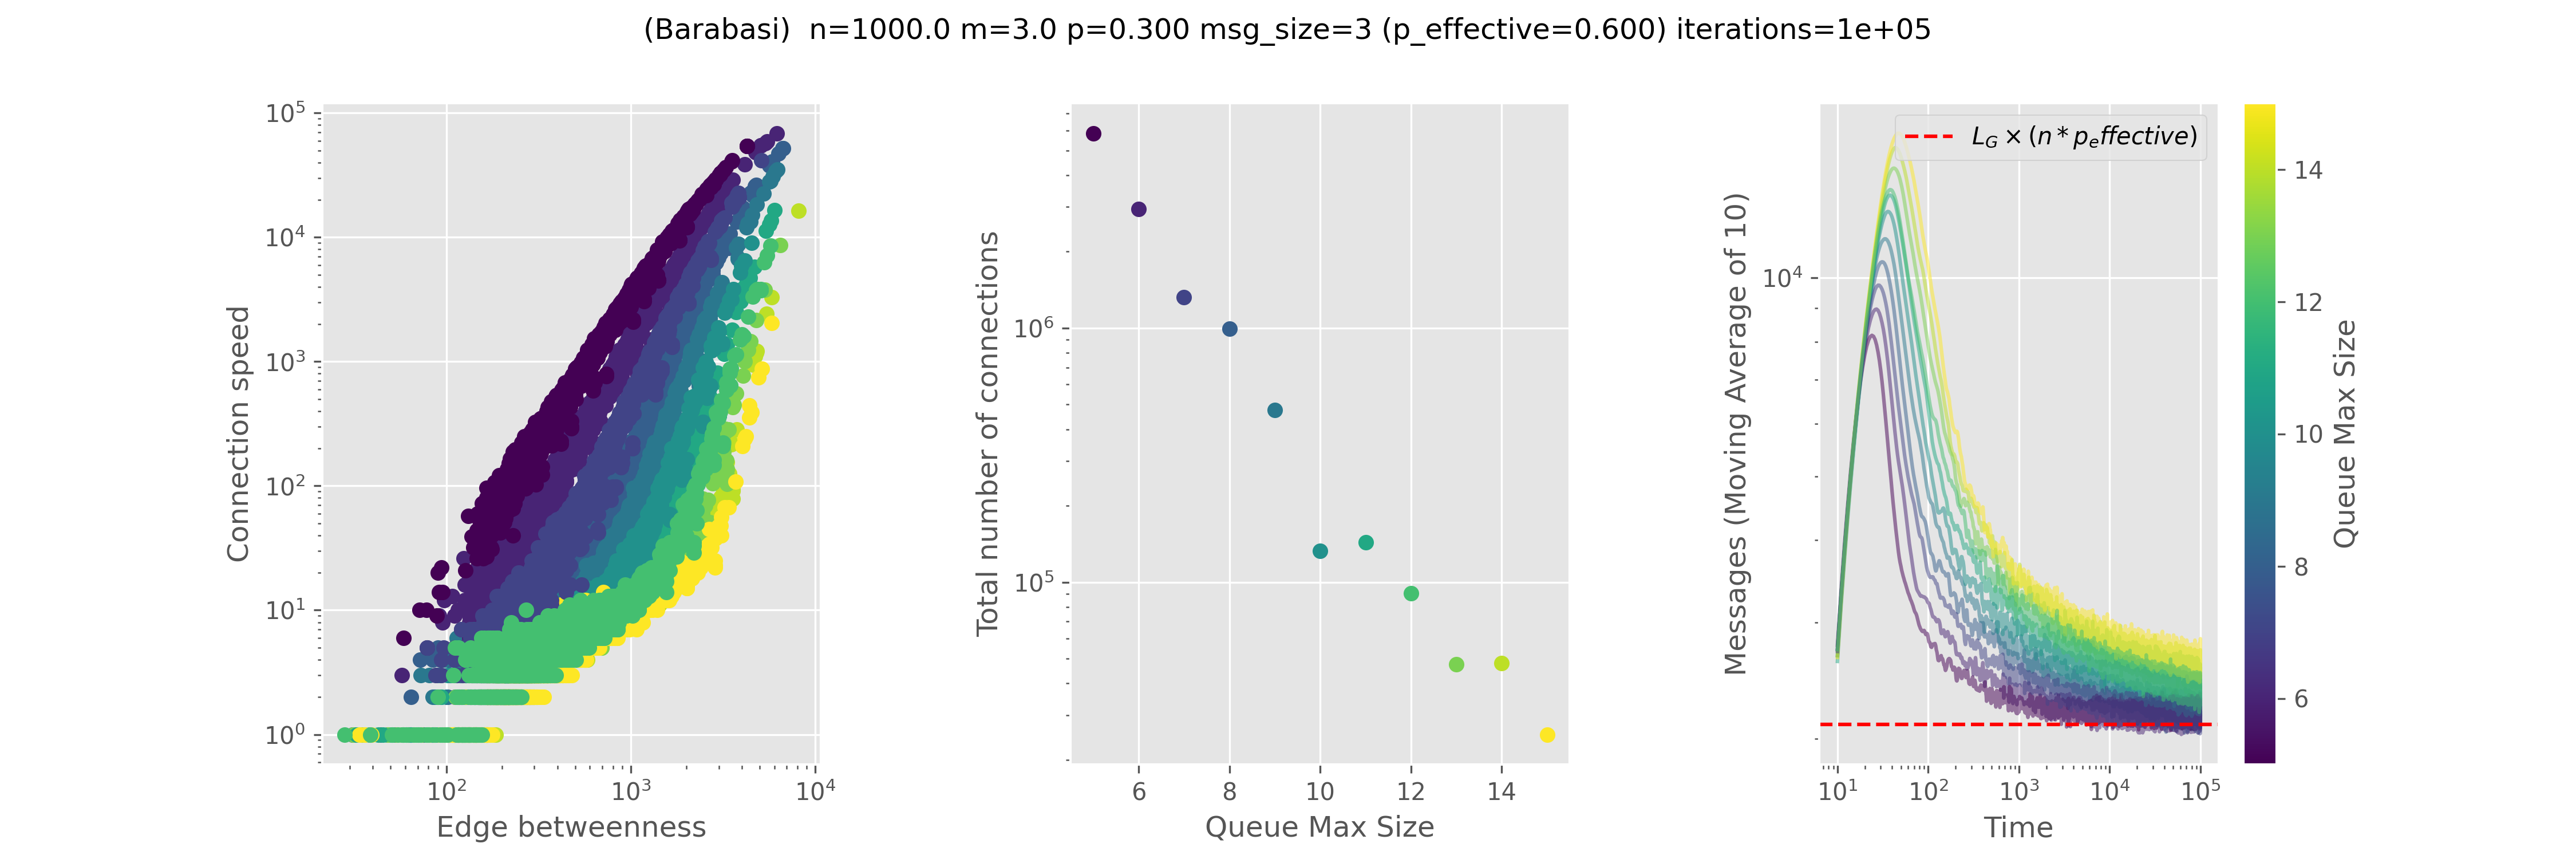
\includegraphics[width=0.8\linewidth]{images/queue_max_size/barabasi_queue_5-15.png}
    \caption{Barabási otimização $k=[5,15]$ }
    \label{fig:enter-label}
\end{figure}

\subsection{(MÉTODO ANTIGO) Erdős}
A análise feito com o modelo Barabási é ainda é mais evidente no modelo de Erdős, uma vez que ele é mais homogêneo em vários parâmetros.



\begin{figure}[H]
    \centering
    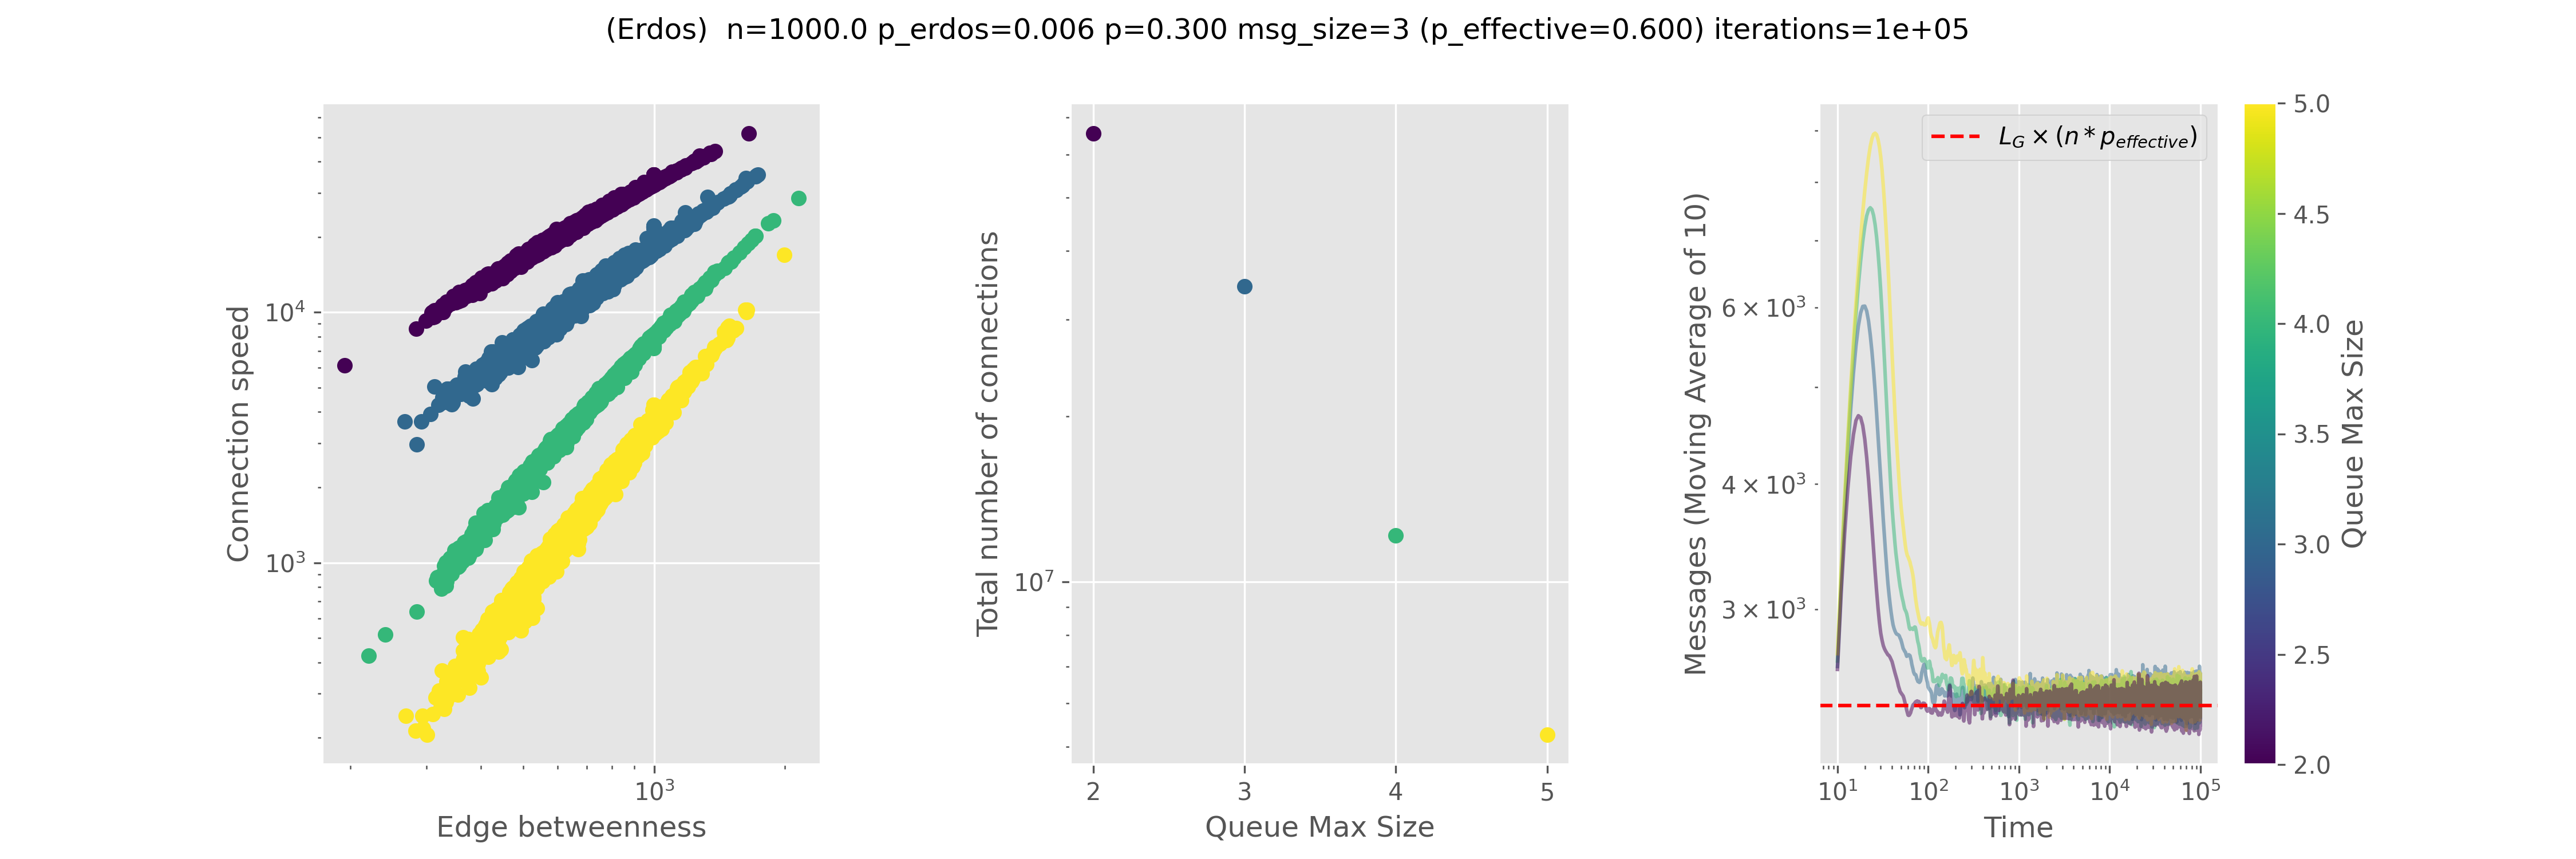
\includegraphics[width=0.8\linewidth]{images/queue_max_size/erdos_queue_2-5.png}
    \caption{Erdős otimização $k=[2,5]$ }
    \label{fig:enter-label}
\end{figure}

\begin{figure}[H]
    \centering
    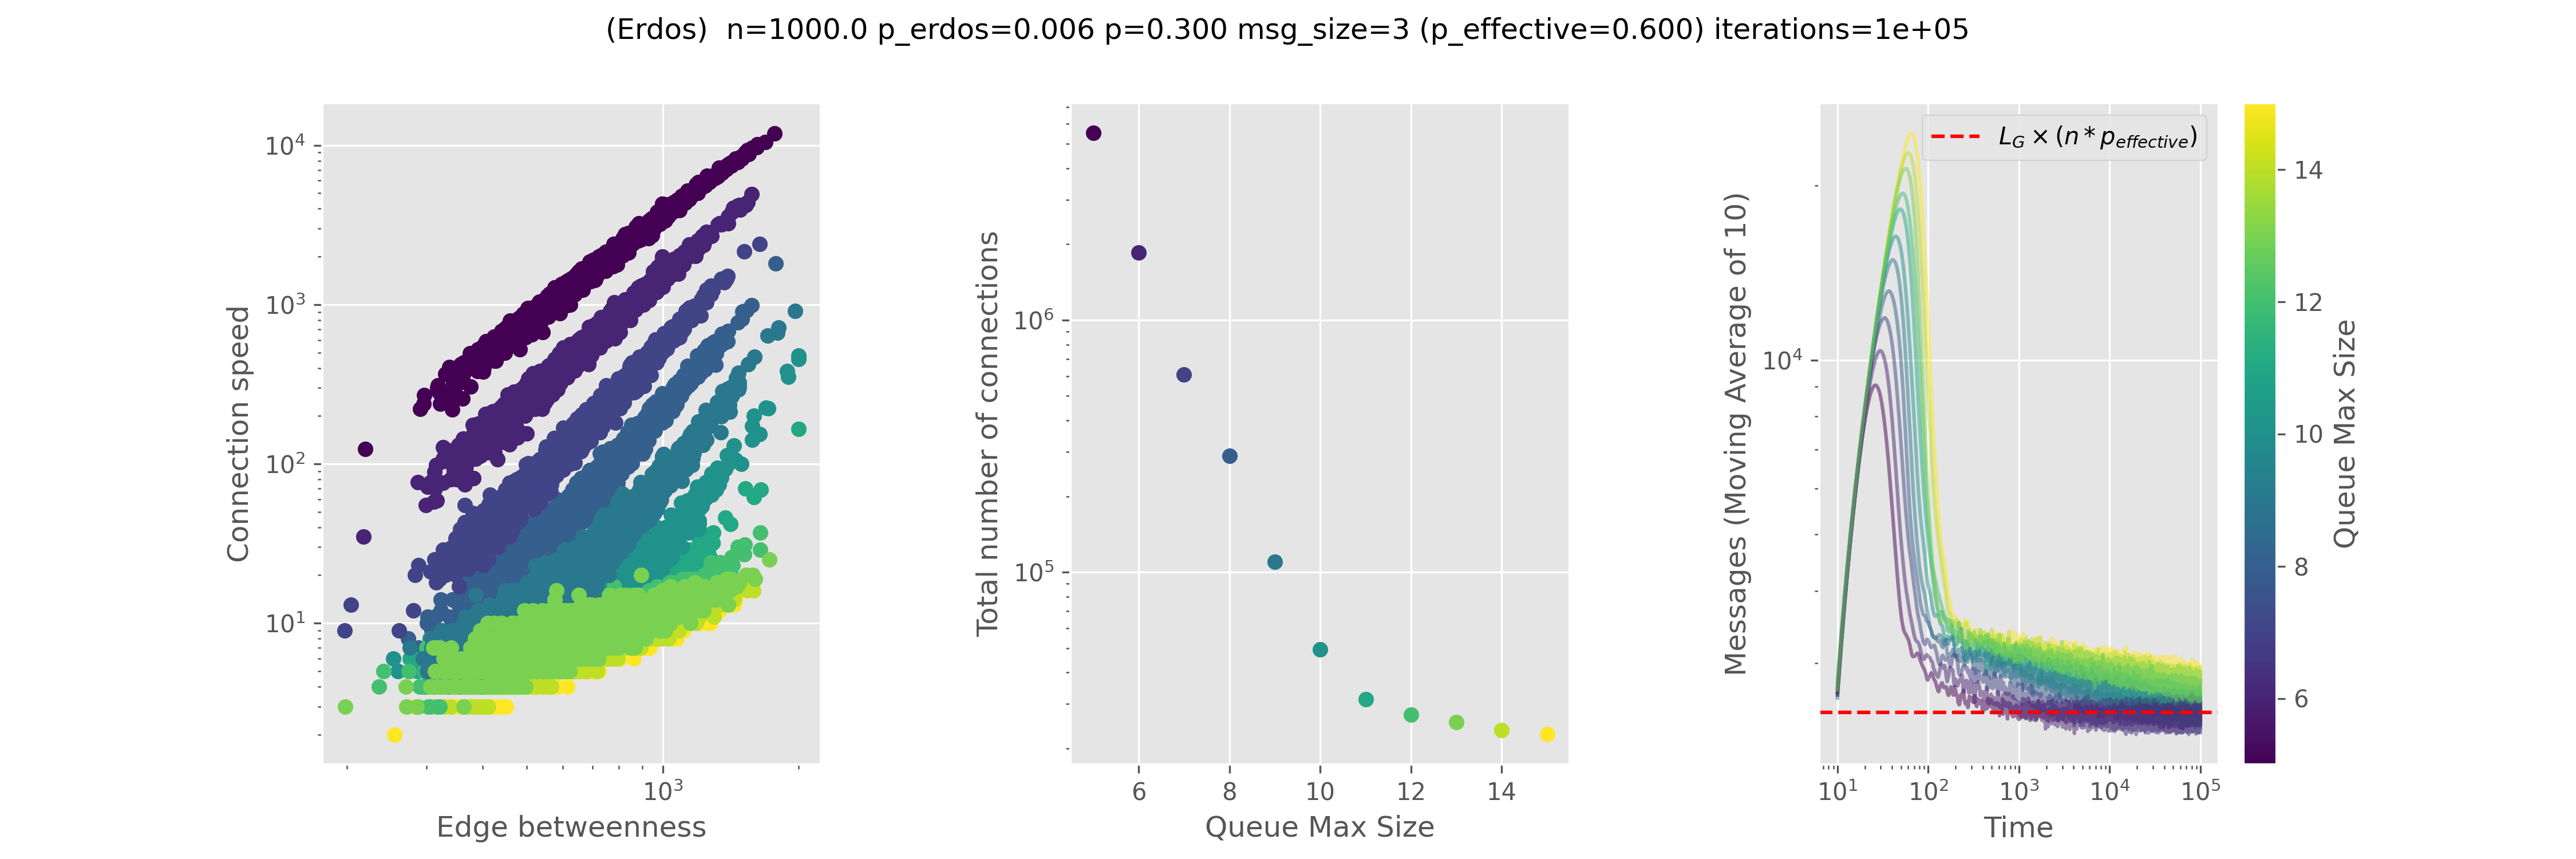
\includegraphics[width=0.8\linewidth]{images/queue_max_size/erdos_queue_5-15.png}
    \caption{Erdős otimização $k=[5,15]$ }
    \label{fig:enter-label}
\end{figure}

\subsection{(MÉTODO ANTIGO) Custo de diferentes topologias}
Com o código atual podemos analisar diferentes topologias e a largura de banda total necessária para manter o trafego abaixo de $k$. Assumindo que o custo para ter uma infraestrutura com essa largura de banda total seja crescente com a mesma, podemos qualitativamente comparar o custo de diferentes topológias

\begin{figure}[H]
    \centering
    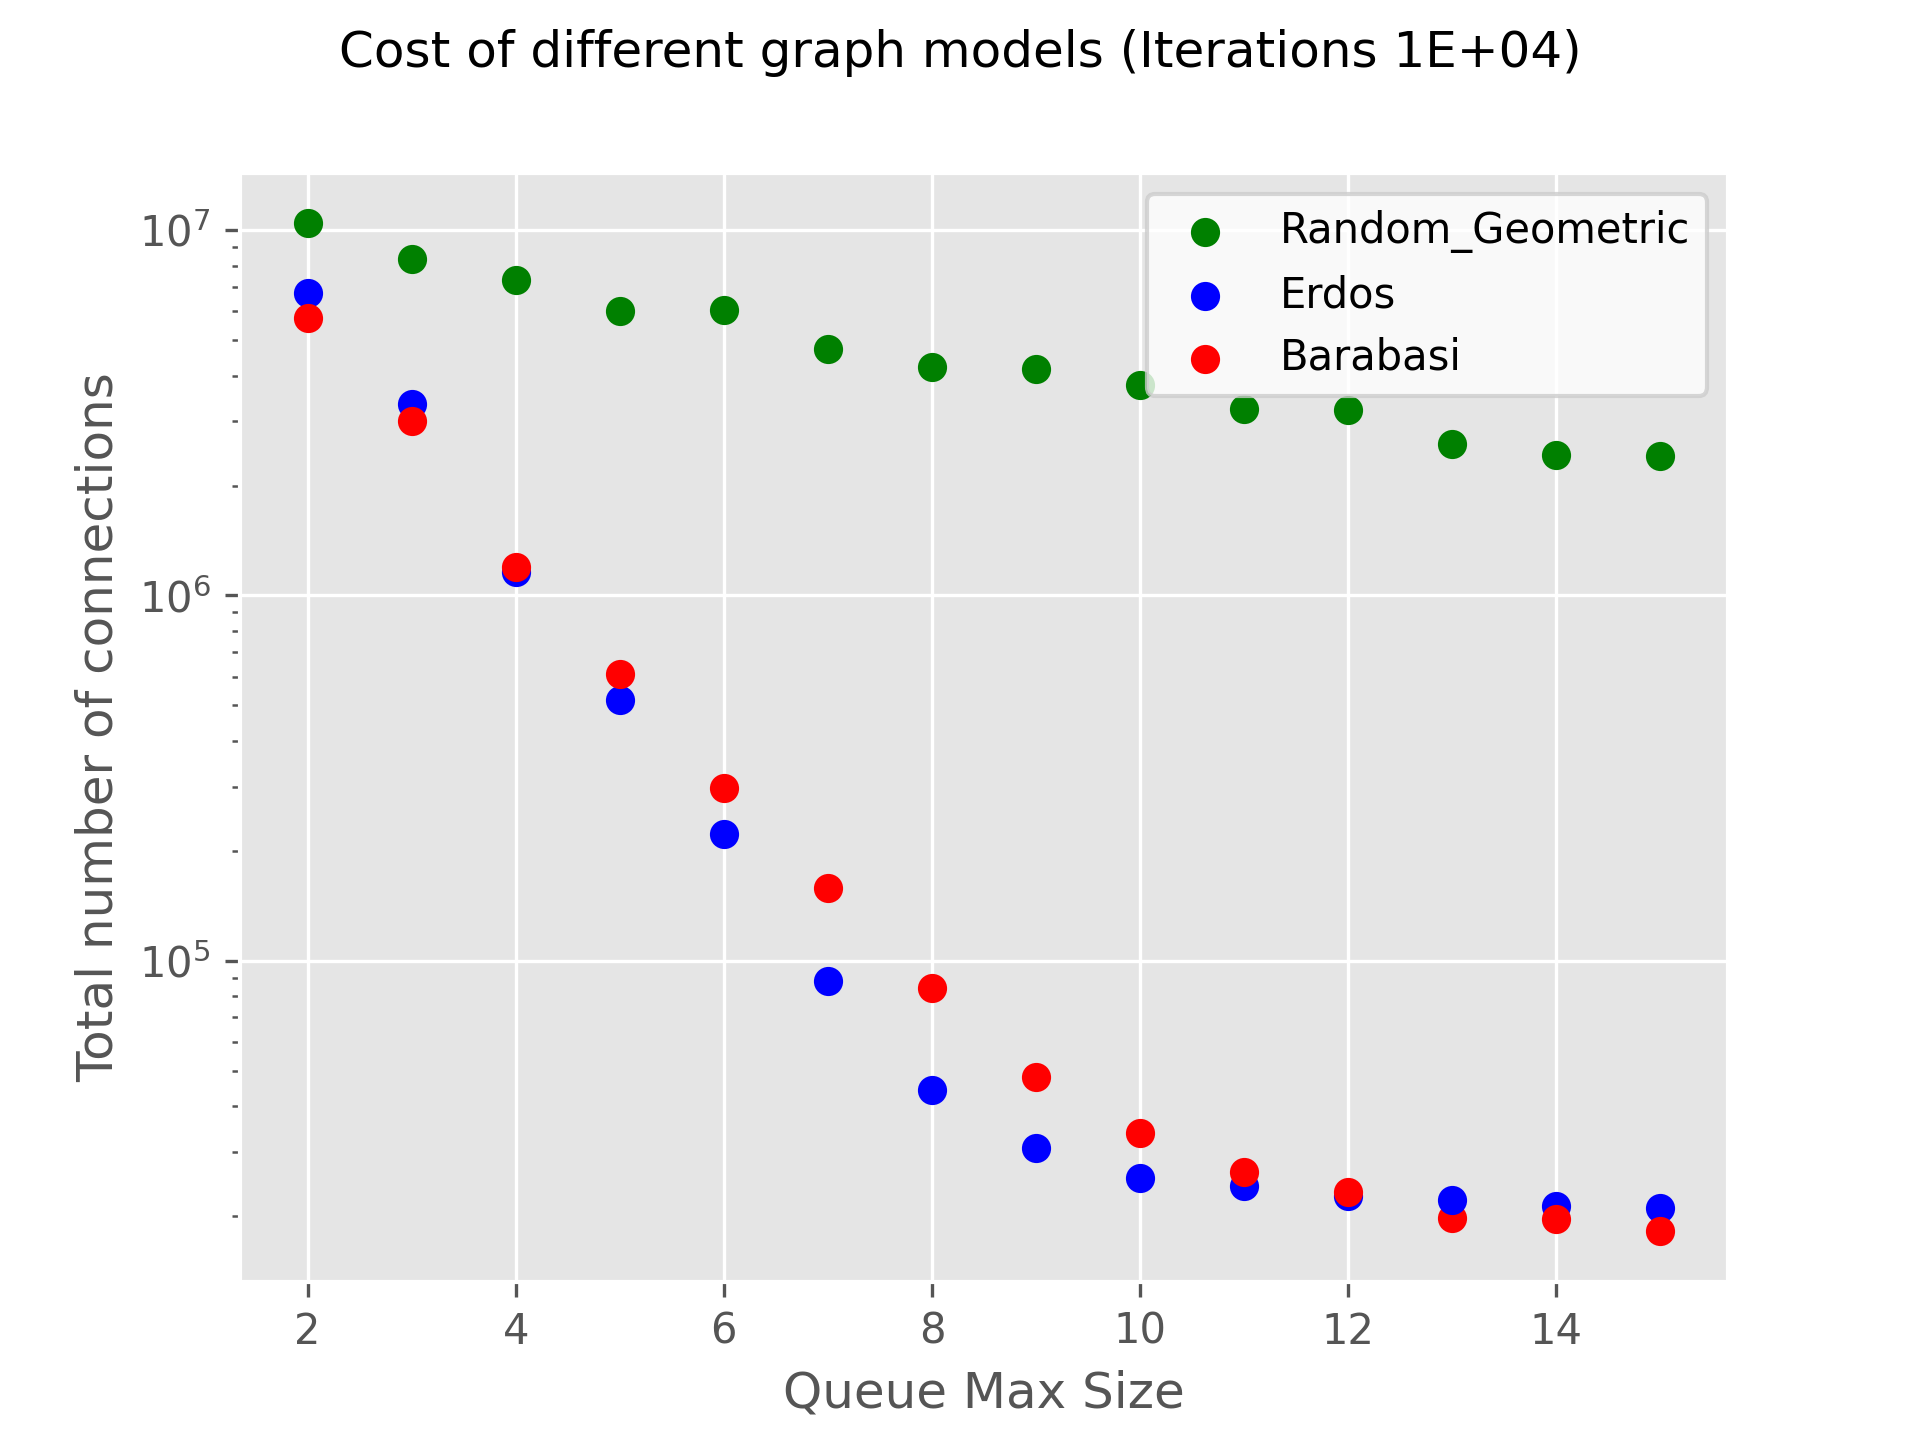
\includegraphics[width=0.8\linewidth]{images/cost_graph_models.png}
    \caption{Custo de diferentes topologias para diferentes $k$ }
    \label{fig:enter-label}
\end{figure}

\section{Simulation optimization techiniques}
Efficient simulation of complex network traffic requires carefully chosen programming techniques. Parallelization within a single simulation is often ineffective due to the highly connected structure of many networks: frequent inter-thread communication introduces substantial performance overhead. To address this limitation, our implementation executes multiple independent simulations in parallel rather than parallelizing each simulation individually.

A common analysis involves fixing the underlying network topology while varying dynamical parameters such as message generation rates or routing strategies. In this context, simulations can share a common cache of distances and routing information. By scheduling simulations with isomorphic graphs to run consecutively, the cache needs to be constructed only once and can be discarded immediately after the final dependent simulation concludes, thereby achieving a significant reduction in memory consumption.


\section{Routing}
A variety of routing strategies can be employed in network systems, in this work, we adopt a strategy based on minimal paths. The implementation begins with the computation of a distance matrix $ D_{ij} $, where each element represents the shortest path length between vertex $ v_i $ and vertex $ v_j $.

Consider a message originating at vertex $ v_i $ with destination at vertex $ v_j $. At each intermediate node $ v_k $, we identify the neighboring vertices of $ v_k $ that are closer to the destination $ v_j $ than $ v_k $ itself. Formally, the set of candidate next vertices to route is defined as:

\begin{equation}
    \text{Next}(v_k, v_j) = \{v \in \text{Neighbors}(v_k) \mid \text{distance}(v, v_j) < \text{distance}(v_k, v_j)\}
\end{equation}

This set defines all valid minimal-path directions that the message can take at the current step. One vertex from this set is then randomly selected, and the message is forwarded to it.
This approach circumvents the need to store all minimal paths between all vertex pairs, which would be highly redundant due to the entanglement of minimal paths—that is, the extensive overlap among shortest paths in complex networks.

Candidate vertices may be pre-calculated with a space complexity of $O(V^2⟨k⟩)$ or computed lazily to conserve memory. While lazy computation avoids large storage requirements, it incurs the runtime overhead of filtering neighbors at every routing step creating a temporary vector to store the candidate vertices. 

Alternatively, we propose an intermediate optimization that stores only the cardinality of valid next vertices in a matrix M.  This allows the algorithm to select a random index x bounded by $M_{i,j}$​ and traverse the neighbor list to locate the corresponding x-th valid node, balancing memory usage with computational speed.


\section{Edge capacity update heuristic}

Let $ G(V, E)$ be a given undirected, strongly connected graph, where each node $v \in V$  generates messages at a fixed rate $R$. Assuming the system operates in a \emph{non-critical regime}—that is, the message generation rates are sufficiently low to avoid congestion—the network reaches a statistical equilibrium. At equilibrium, each edge $ e_i \in E $ is associated with a probability distribution function (PDF), denoted $e_i.\text{TrafficPDF}$, representing the distribution of the number of messages in the queue at any given instant.

We define the \emph{Free Flow Rate} (FFR) of an edge as the proportion of time that the number of queued messages does not exceed the edge’s capacity. Formally, for edge $ e_i $, this is given by:
$$
e_i.\text{FFR} = \mathbb{P}(\text{queue size} \leq e_i.\text{capacity}) =e_i.\text{TrafficCDF}(e_i.\text{capacity}),
$$
where $e_i. \text{TrafficCDF} $ is the cumulative distribution function derived from $ e_i.\text{TrafficPDF} $.

Given a desired minimum free flow rate, denoted $ \text{FFR}_{\text{desired}} $, our objective is to determine a capacity configuration $ \{e.\text{capacity} \mid e \in E\} $ such that:
\begin{itemize}
    \item Each edge satisfies $ e_i.\text{FFR}\geq \text{FFR}_{\text{desired}} $, and
    \item The total capacity $ \sum_{e \in E} e.\text{capacity} $ is minimized.
\end{itemize}

To this end, we let the system evolve for a sufficiently long time interval $ \Delta T $, allowing it to reach equilibrium. We then estimate $e_i.\text{TrafficPDF}$ for each edge and compute the minimal capacity required to achieve the desired FFR using the rule:
\begin{equation}
\label{eq:method}
\forall e \in E, \quad e.\text{capacity} = \min \left\{ x \in \mathbb{N} \;\middle|\; e.\text{TrafficCDF}(x) \geq \text{FFR}_{\text{desired}} \right\}.
\end{equation}

This procedure acts as a \emph{heuristic}, since altering the capacity of one edge may affect the traffic distribution across the entire network. However, by iteratively applying Equation~\eqref{eq:method}, allowing the system to re-stabilize over successive intervals $ \Delta T $, we empirically observe convergence toward a stable configuration that satisfies the FFR constraint while minimizing the total capacity.

\begin{figure}[H]
    \centering
    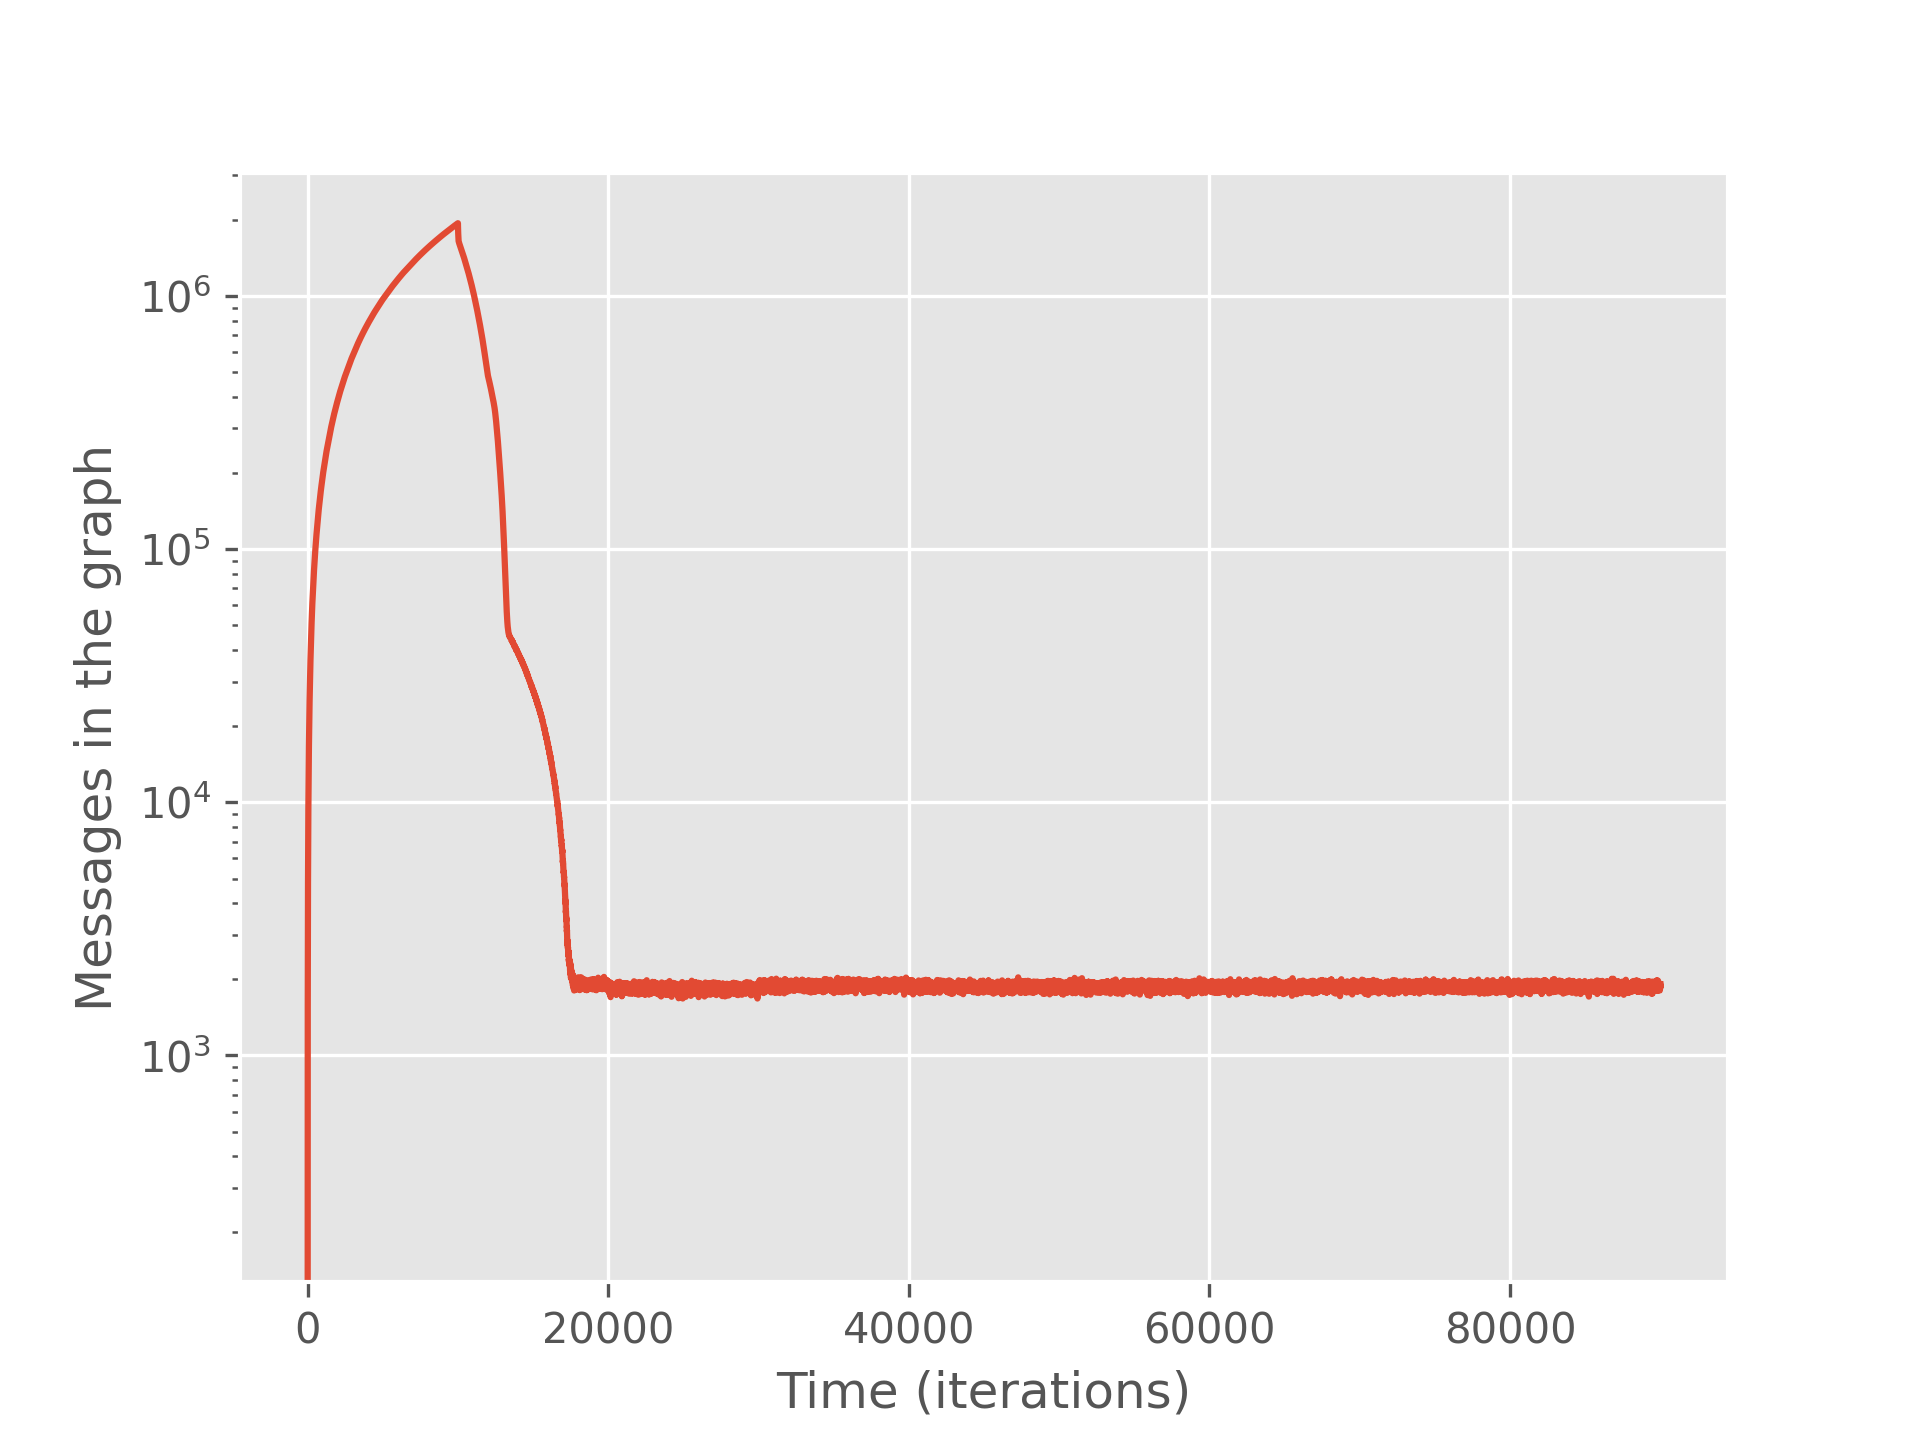
\includegraphics[width=0.8\linewidth]{images/10times_the_method_messages_x_time__sha1__e01d7a5f5938bfa367f026f13276f693ef086a2f.png}
    \label{fig:enter-label}
\end{figure}

\begin{figure}[H]
    \centering
    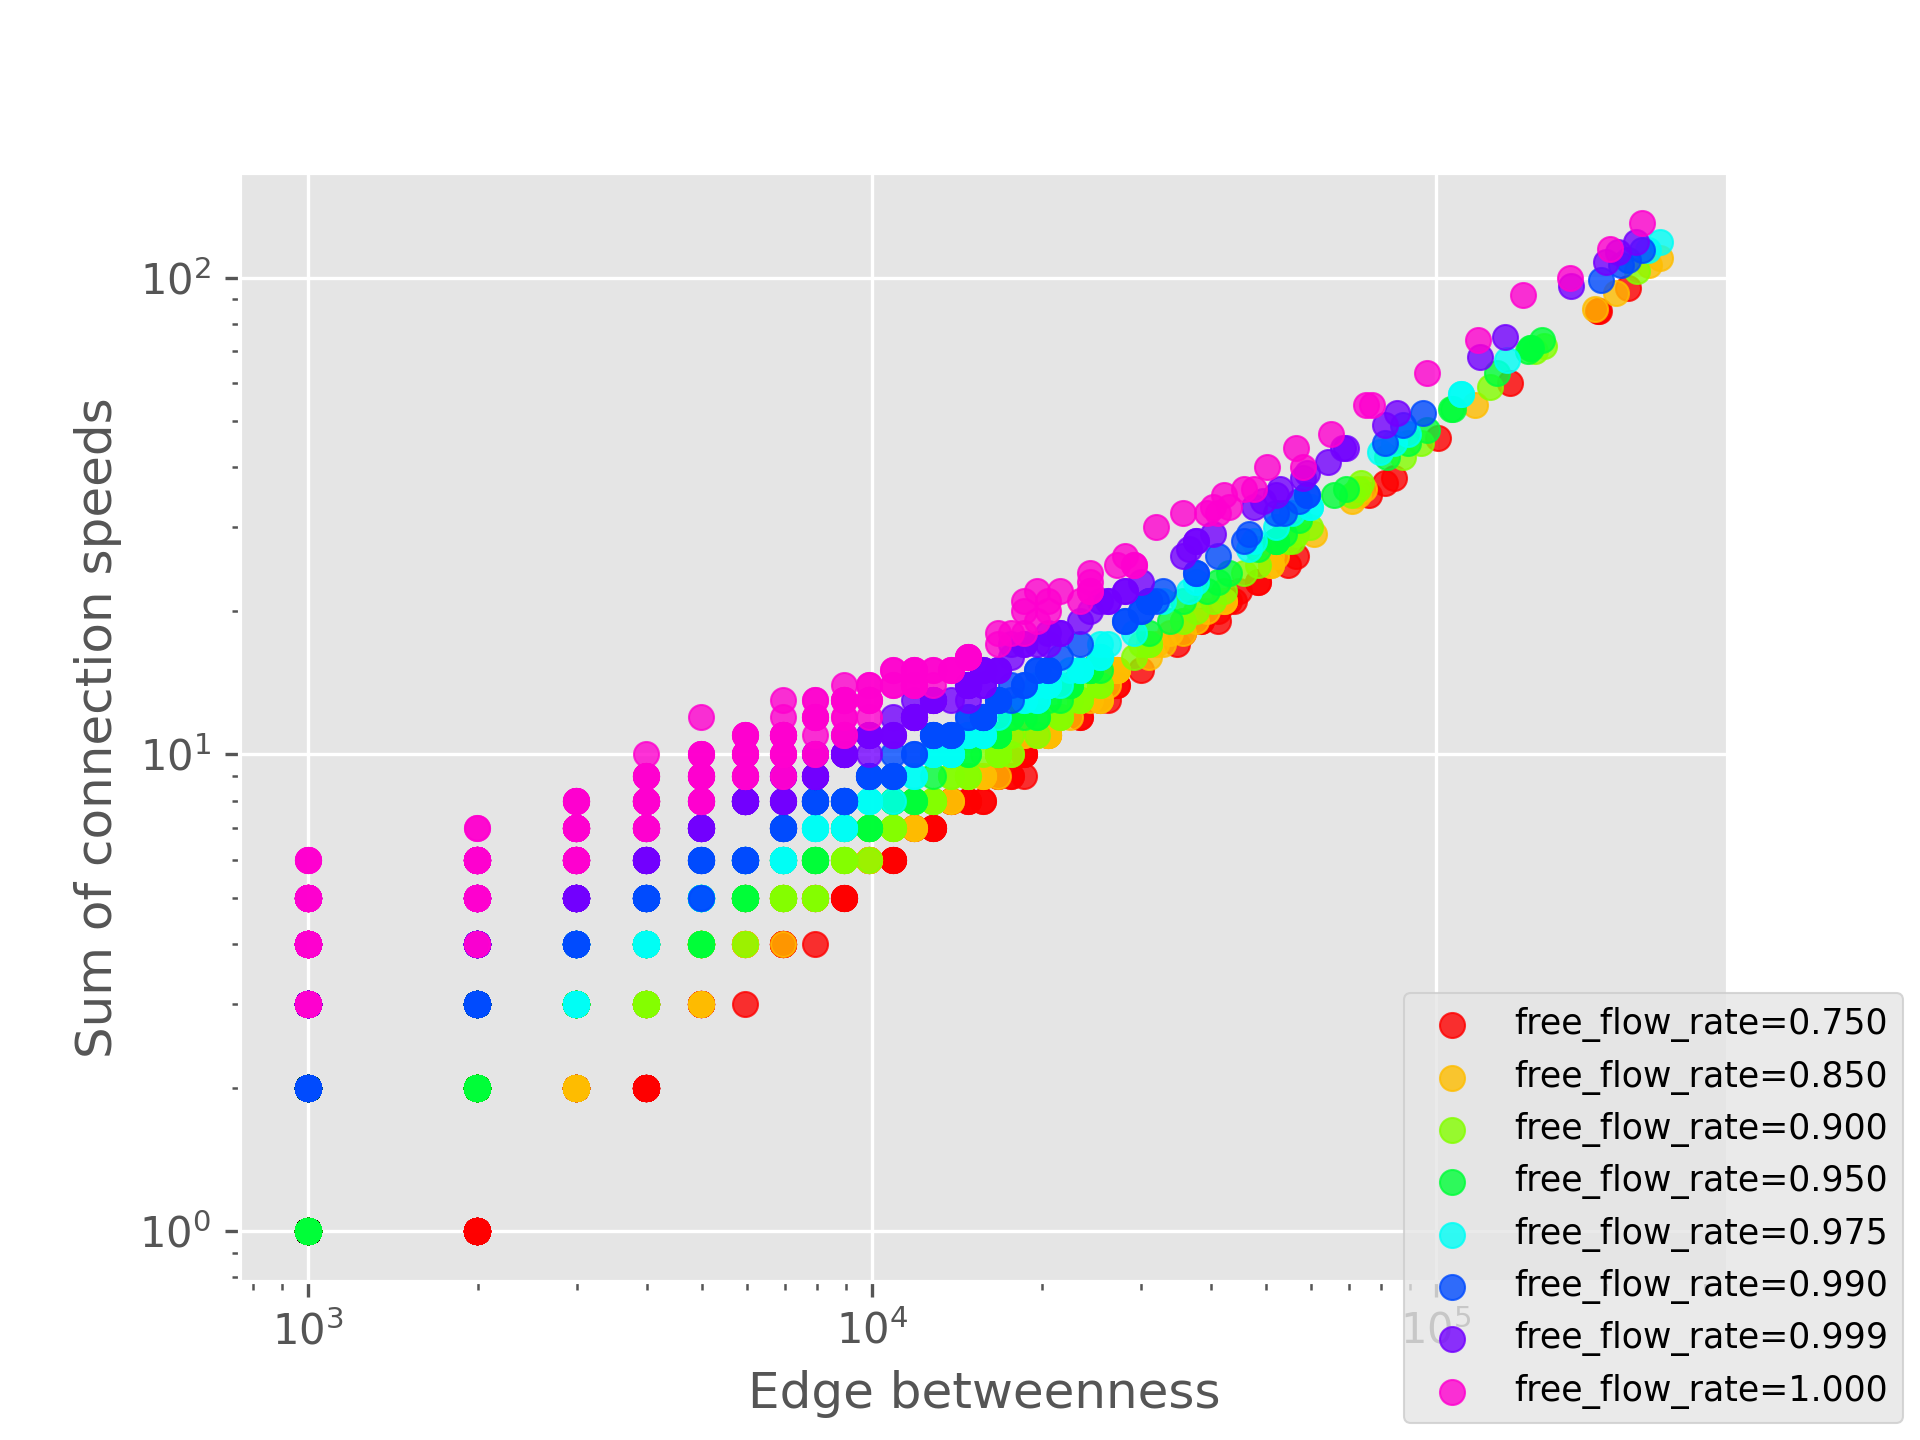
\includegraphics[width=0.8\linewidth]{images/different_free_flow_rates_edge_betweenness__sha1__f5229b8a1a3d52443c76540cd86e3d4accd374de (copy).png}
    \label{fig:enter-label}
\end{figure}

\begin{figure}[H]
    \centering
    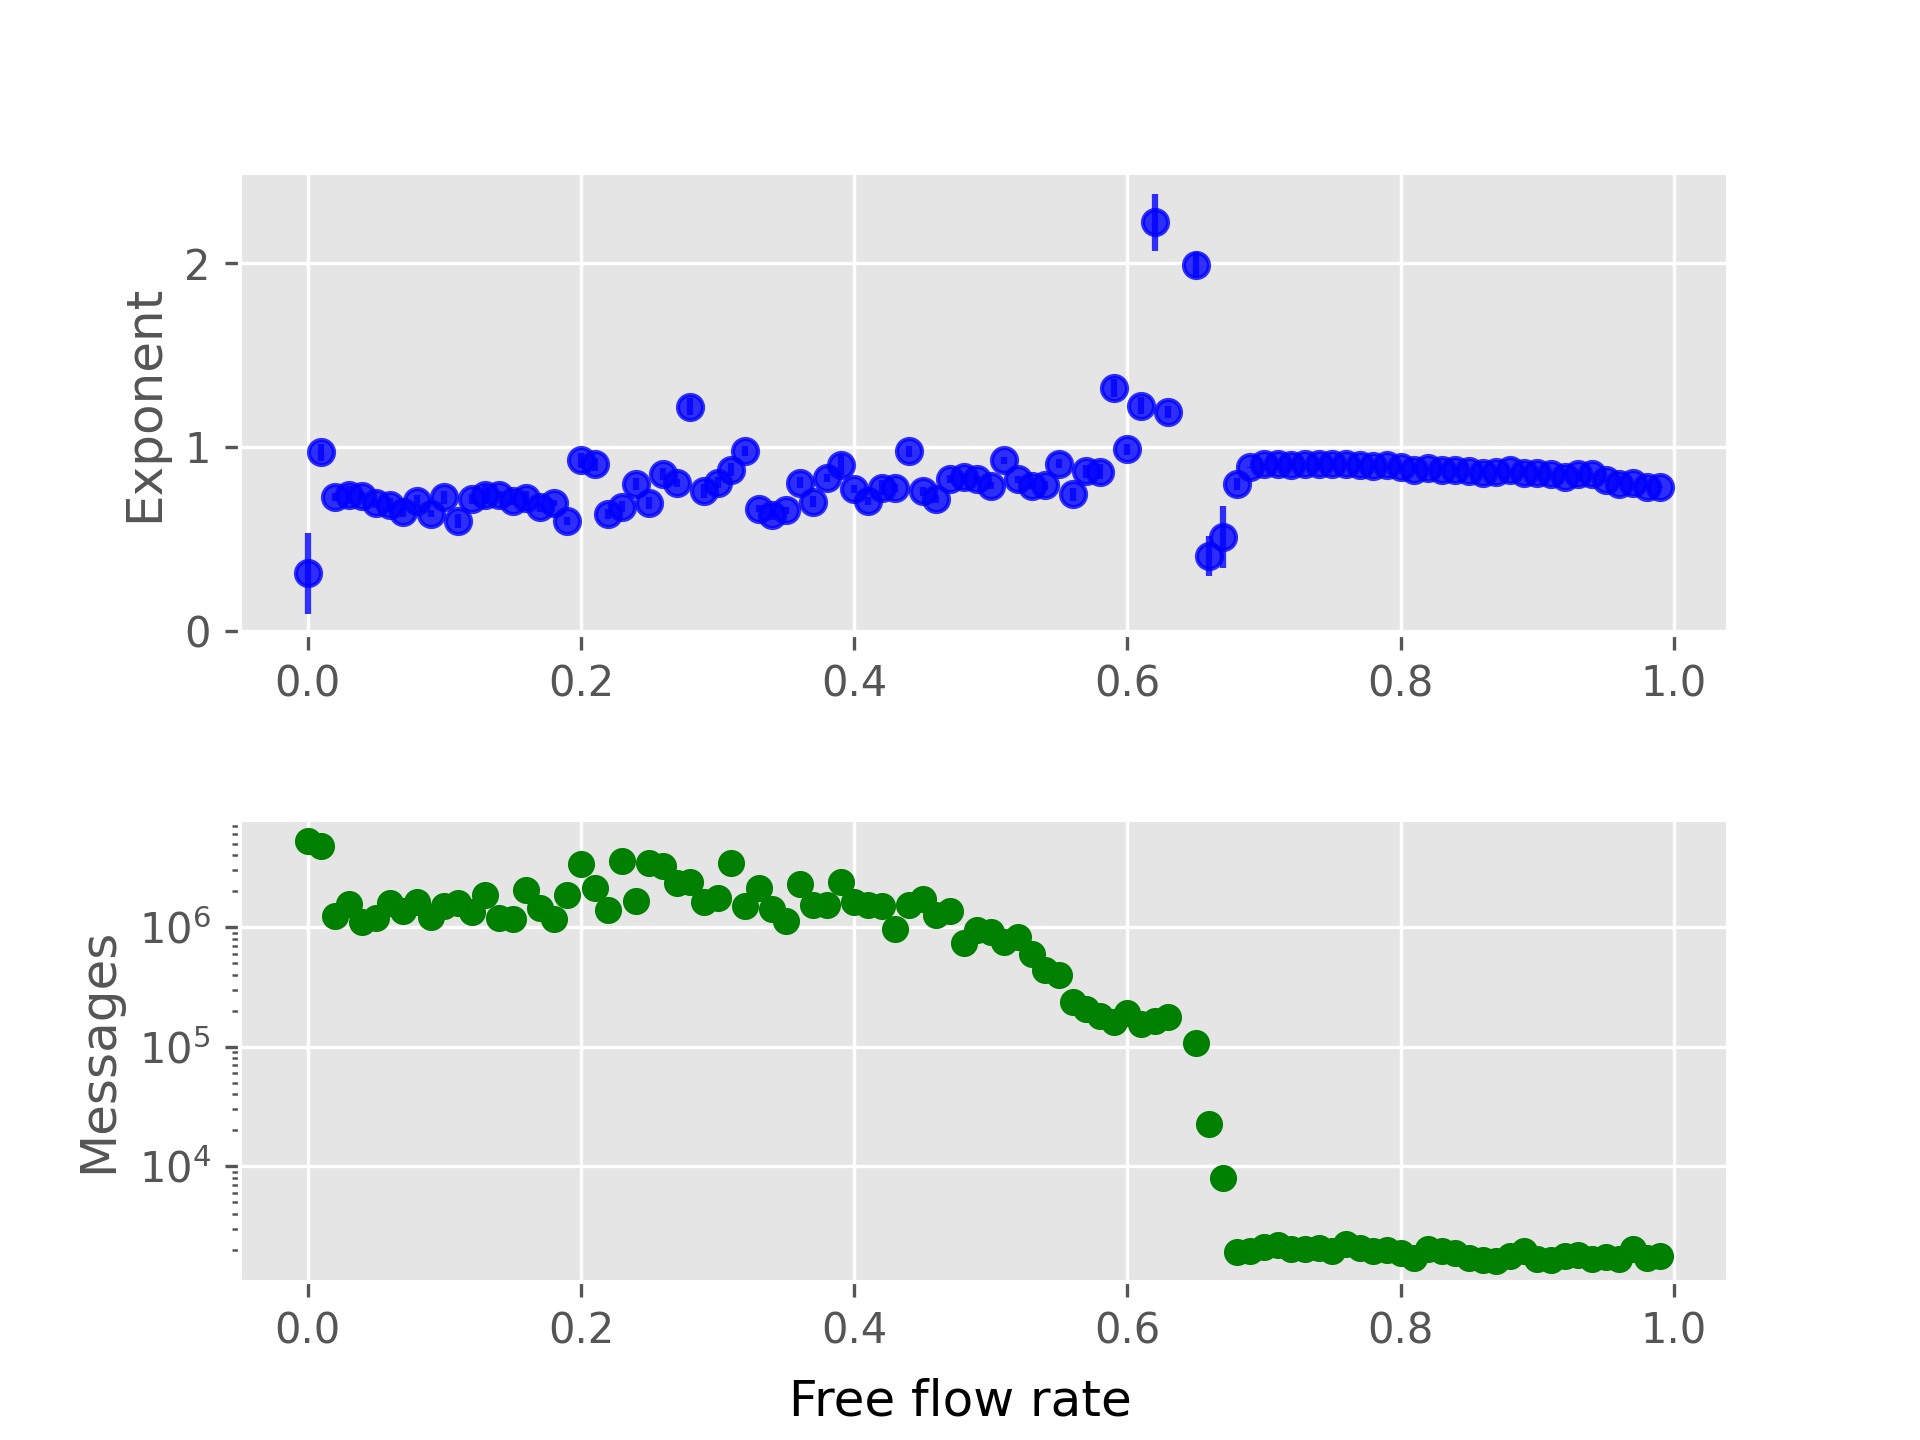
\includegraphics[width=0.8\linewidth]{images/tmp_edge_betweenness__sha1__06f93401145c2f645e02d916f6da493aceb2007a.png}
    \label{fig:enter-label}
\end{figure}

\section{Configuration Model}
We made a fitting of the edge betweeness vs the capacity found by the method.

A configuration model was used of a graph with powerlaw degree $\gamma$ 

\begin{figure}[H]
    \centering
    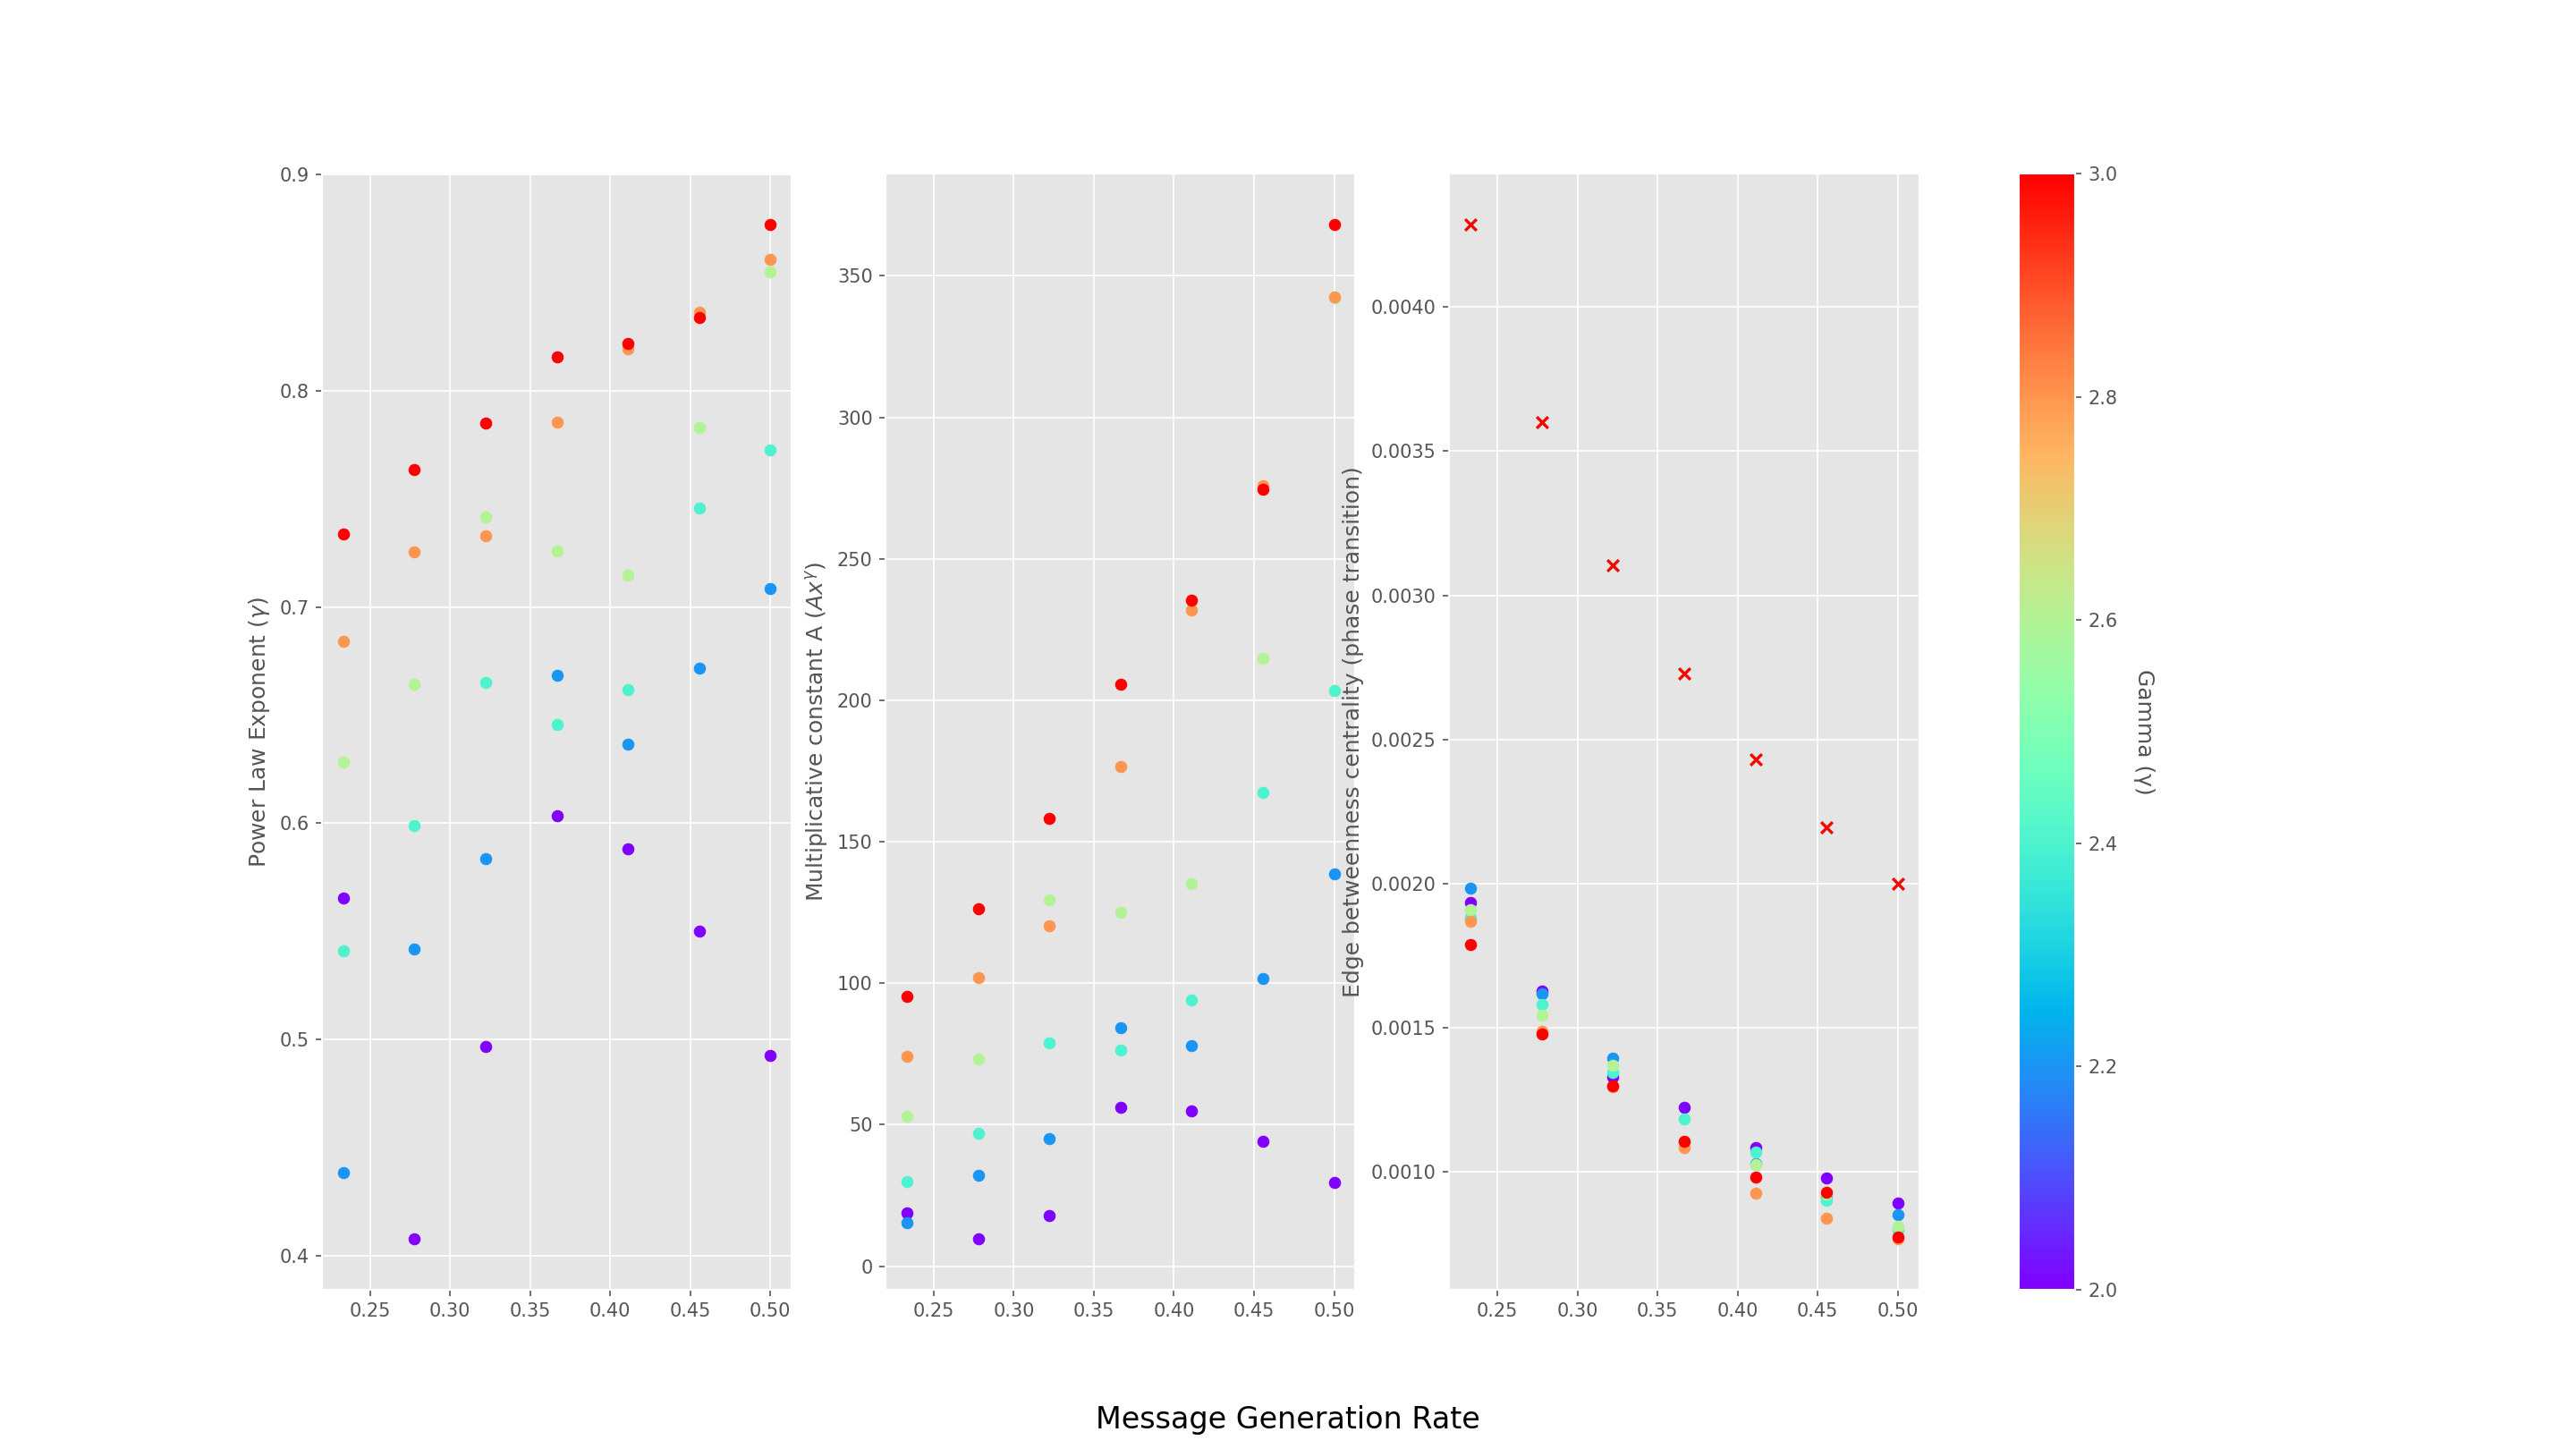
\includegraphics[width=0.8\linewidth]{images/fitted_values.png}
\end{figure}

\section{Correlations under Varying Visibility}

In the unconstrained traffic regime (where link capacities are effectively infinite), varying the routing visibility, denoted as $r$, reveals two limiting analytical cases:

\begin{itemize}
    \item \textbf{Optimal Shortest-Path Routing:} In this limit, every message traverses a minimal path. By the definition of \textit{edge betweenness centrality}, this implies that the flux of messages through an edge is exactly proportional to its betweenness.
    \item \textbf{Random Walk Routing:} In this limit, every edge is visited with equal probability. Consequently, the average message flux on an edge is constant. For a vertex, the load is proportional to the number of incident edges (its degree).
\end{itemize}

\begin{figure}[H]
    \centering
    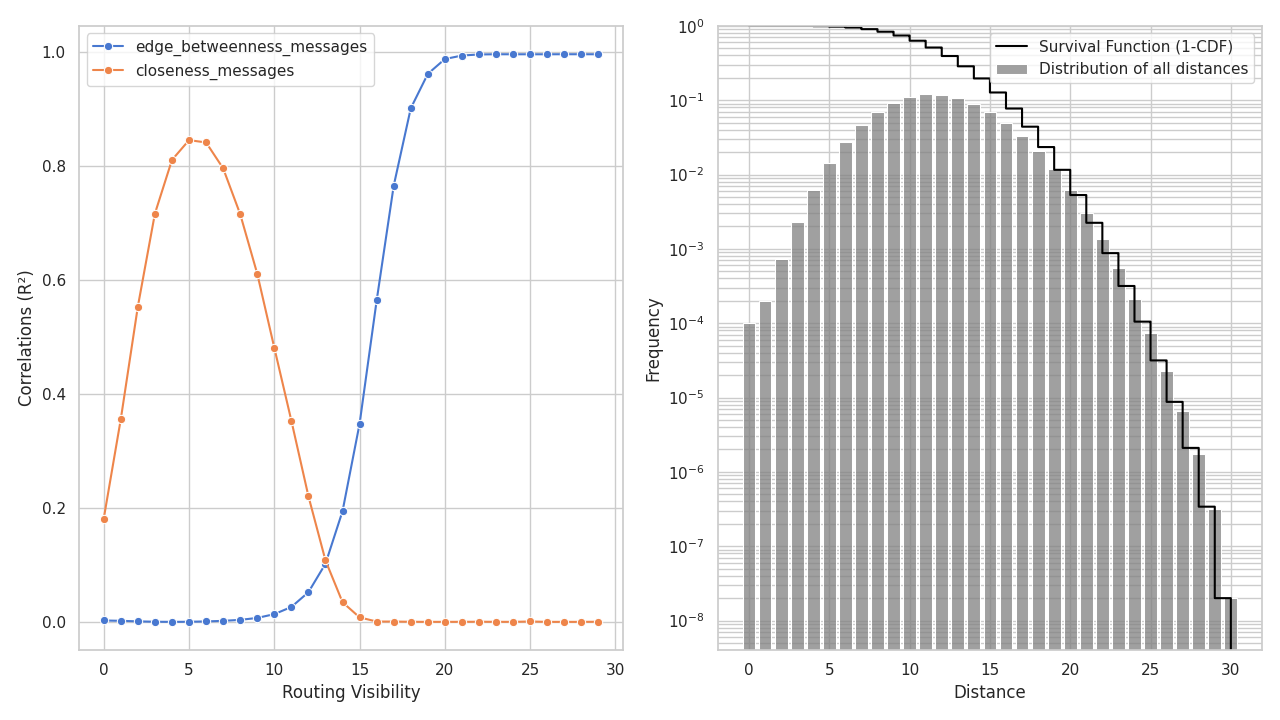
\includegraphics[width=0.8\linewidth]{images/correlations.png}
\end{figure}


When analyzing the correlation between visibility and edge betweenness, the results align with theoretical expectations. For small $r$, there is no significant correlation. However, as $r$ increases sufficiently such that the distance between nodes rarely exceeds $r$ (a property observable via the distance \textit{survival function}), the correlation converges to 1.

Conversely, the relationship between visibility and the correlation of \textit{closeness centrality} with node load yields non-trivial results. Vertices that possess high closeness centrality—those on average closer to all other nodes—are statistically more likely to intercept messages routed via minimal paths.

\section{Standard Deviation of messages arrival}
Given that the source-destination pairs are chosen uniformly at random and messages are created with probability $\rho$, the flux of messages through a specific edge follows a Poisson distribution. A fundamental property of Poissonian processes is that the variance equals the mean ($\sigma^2 = \mu$). Consequently, the standard deviation is given by:

\begin{equation}
    \sigma = \sqrt{\mu} = \sqrt{N \rho b}
\end{equation}

Our simulation data implies a strong fit with this expectation, confirming the stochastic nature of the traffic distribution.
\begin{figure}[H]
    \centering
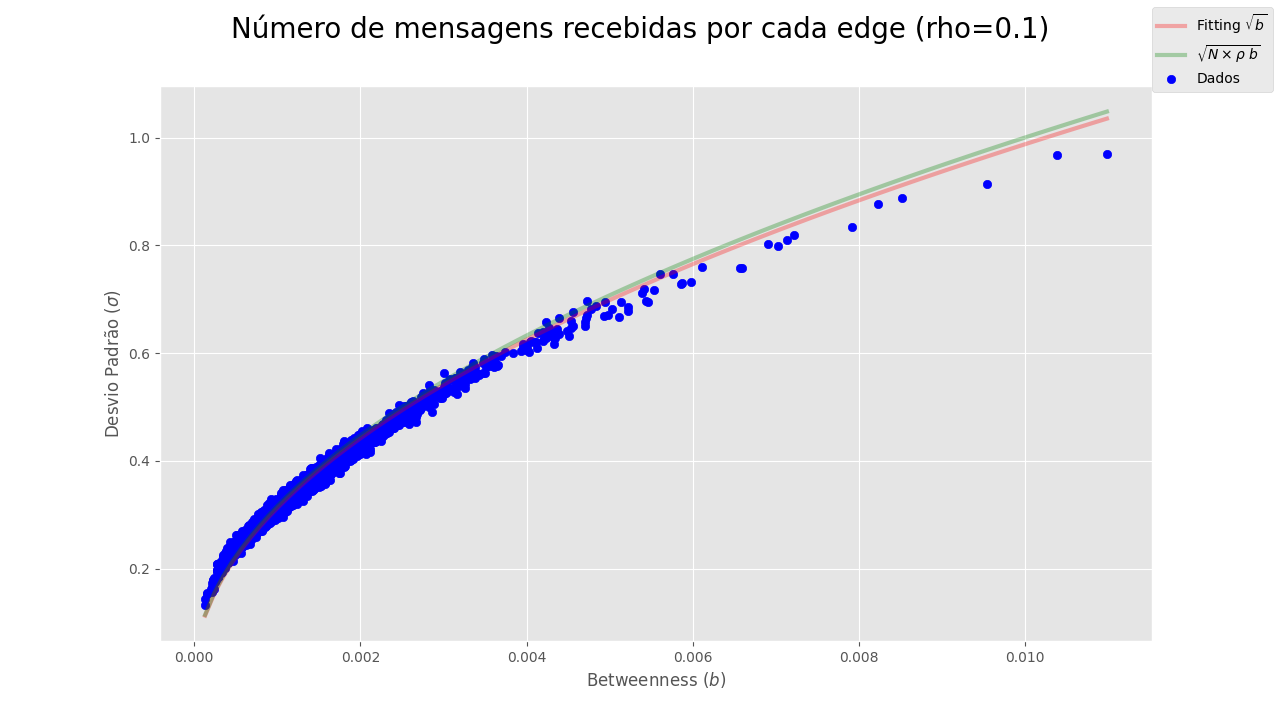
\includegraphics[width=0.8\linewidth]{images/poisson_0.1.png}
\end{figure}


\begin{figure}[H]
    \centering
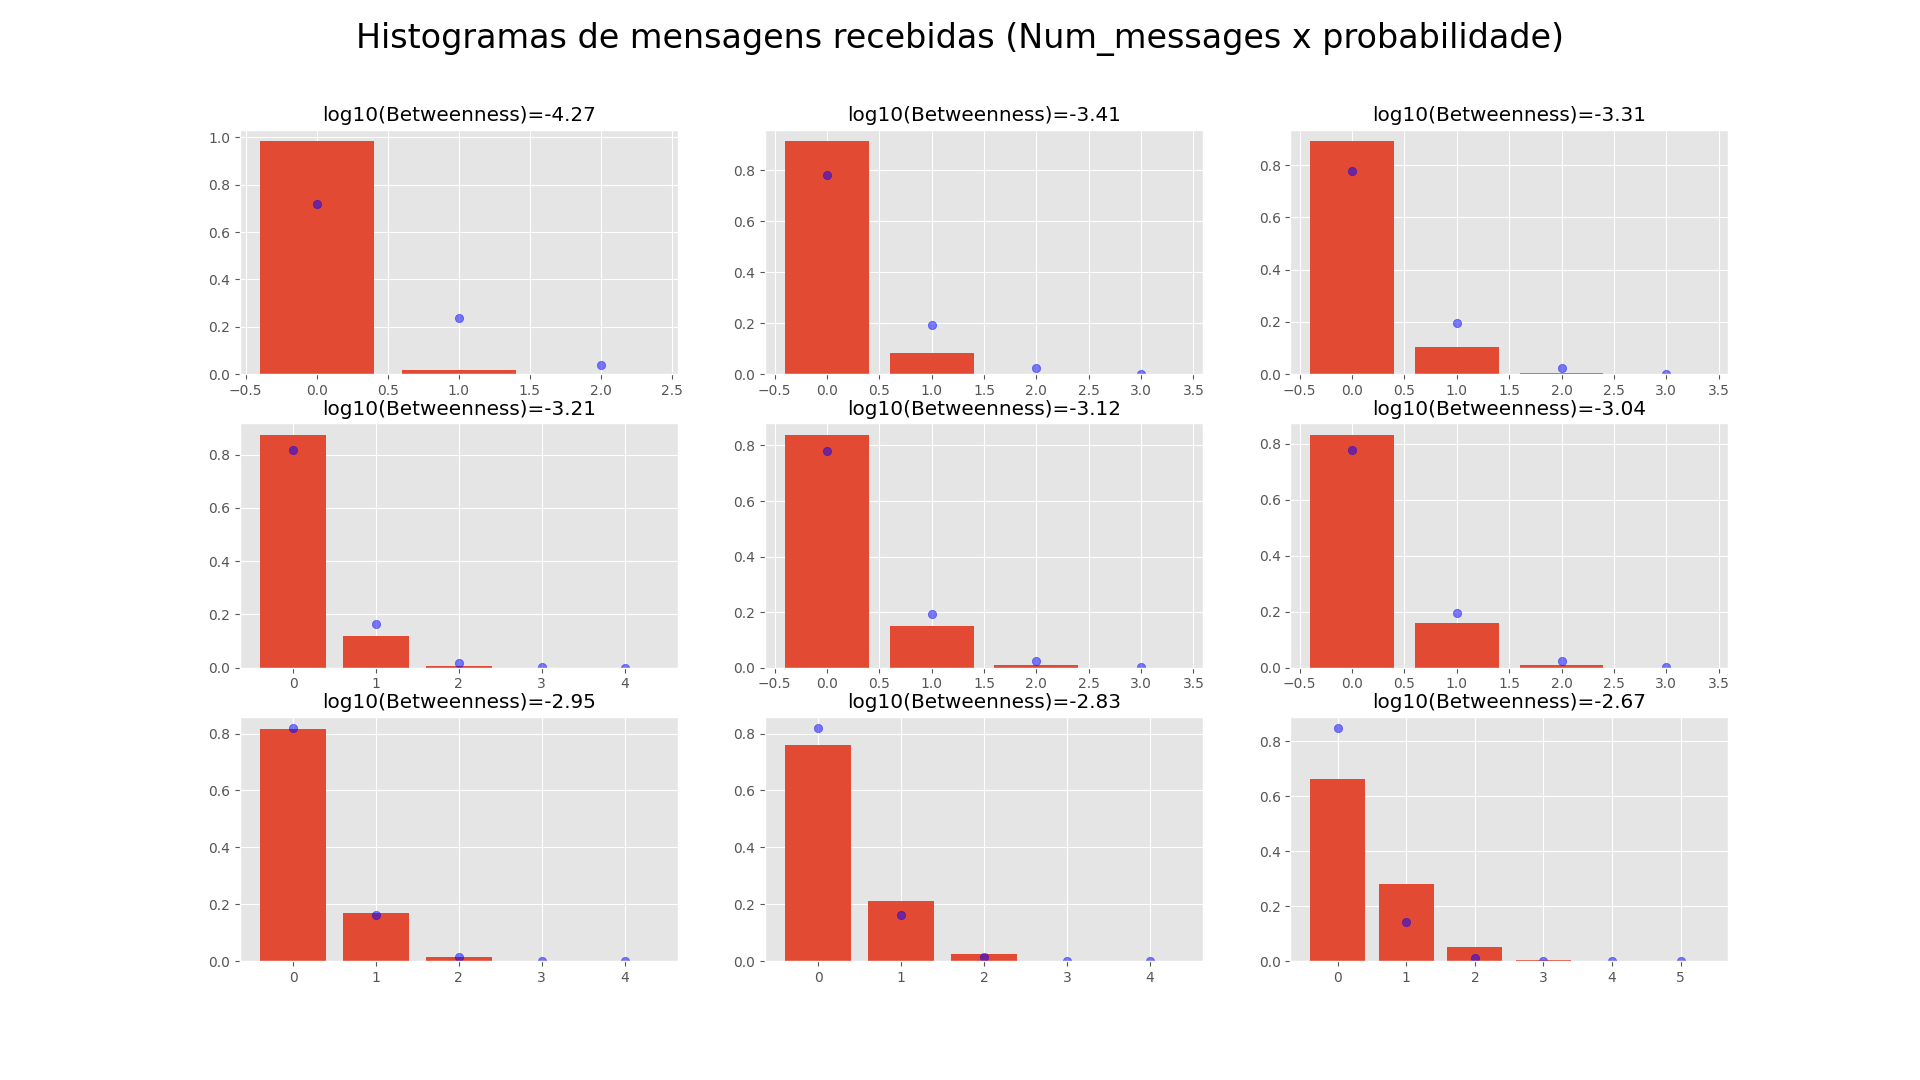
\includegraphics[width=0.8\linewidth]{images/histogramas.png}
\end{figure}



\end{document}
